% Options for packages loaded elsewhere
\PassOptionsToPackage{unicode}{hyperref}
\PassOptionsToPackage{hyphens}{url}
%
\documentclass[
]{article}
\usepackage{lmodern}
\usepackage{amssymb,amsmath}
\usepackage{ifxetex,ifluatex}
\ifnum 0\ifxetex 1\fi\ifluatex 1\fi=0 % if pdftex
  \usepackage[T1]{fontenc}
  \usepackage[utf8]{inputenc}
  \usepackage{textcomp} % provide euro and other symbols
\else % if luatex or xetex
  \usepackage{unicode-math}
  \defaultfontfeatures{Scale=MatchLowercase}
  \defaultfontfeatures[\rmfamily]{Ligatures=TeX,Scale=1}
\fi
% Use upquote if available, for straight quotes in verbatim environments
\IfFileExists{upquote.sty}{\usepackage{upquote}}{}
\IfFileExists{microtype.sty}{% use microtype if available
  \usepackage[]{microtype}
  \UseMicrotypeSet[protrusion]{basicmath} % disable protrusion for tt fonts
}{}
\makeatletter
\@ifundefined{KOMAClassName}{% if non-KOMA class
  \IfFileExists{parskip.sty}{%
    \usepackage{parskip}
  }{% else
    \setlength{\parindent}{0pt}
    \setlength{\parskip}{6pt plus 2pt minus 1pt}}
}{% if KOMA class
  \KOMAoptions{parskip=half}}
\makeatother
\usepackage{xcolor}
\IfFileExists{xurl.sty}{\usepackage{xurl}}{} % add URL line breaks if available
\IfFileExists{bookmark.sty}{\usepackage{bookmark}}{\usepackage{hyperref}}
\hypersetup{
  pdftitle={R Module 2},
  pdfauthor={Connor Gibbs},
  hidelinks,
  pdfcreator={LaTeX via pandoc}}
\urlstyle{same} % disable monospaced font for URLs
\usepackage[margin=1in]{geometry}
\usepackage{color}
\usepackage{fancyvrb}
\newcommand{\VerbBar}{|}
\newcommand{\VERB}{\Verb[commandchars=\\\{\}]}
\DefineVerbatimEnvironment{Highlighting}{Verbatim}{commandchars=\\\{\}}
% Add ',fontsize=\small' for more characters per line
\usepackage{framed}
\definecolor{shadecolor}{RGB}{248,248,248}
\newenvironment{Shaded}{\begin{snugshade}}{\end{snugshade}}
\newcommand{\AlertTok}[1]{\textcolor[rgb]{0.94,0.16,0.16}{#1}}
\newcommand{\AnnotationTok}[1]{\textcolor[rgb]{0.56,0.35,0.01}{\textbf{\textit{#1}}}}
\newcommand{\AttributeTok}[1]{\textcolor[rgb]{0.77,0.63,0.00}{#1}}
\newcommand{\BaseNTok}[1]{\textcolor[rgb]{0.00,0.00,0.81}{#1}}
\newcommand{\BuiltInTok}[1]{#1}
\newcommand{\CharTok}[1]{\textcolor[rgb]{0.31,0.60,0.02}{#1}}
\newcommand{\CommentTok}[1]{\textcolor[rgb]{0.56,0.35,0.01}{\textit{#1}}}
\newcommand{\CommentVarTok}[1]{\textcolor[rgb]{0.56,0.35,0.01}{\textbf{\textit{#1}}}}
\newcommand{\ConstantTok}[1]{\textcolor[rgb]{0.00,0.00,0.00}{#1}}
\newcommand{\ControlFlowTok}[1]{\textcolor[rgb]{0.13,0.29,0.53}{\textbf{#1}}}
\newcommand{\DataTypeTok}[1]{\textcolor[rgb]{0.13,0.29,0.53}{#1}}
\newcommand{\DecValTok}[1]{\textcolor[rgb]{0.00,0.00,0.81}{#1}}
\newcommand{\DocumentationTok}[1]{\textcolor[rgb]{0.56,0.35,0.01}{\textbf{\textit{#1}}}}
\newcommand{\ErrorTok}[1]{\textcolor[rgb]{0.64,0.00,0.00}{\textbf{#1}}}
\newcommand{\ExtensionTok}[1]{#1}
\newcommand{\FloatTok}[1]{\textcolor[rgb]{0.00,0.00,0.81}{#1}}
\newcommand{\FunctionTok}[1]{\textcolor[rgb]{0.00,0.00,0.00}{#1}}
\newcommand{\ImportTok}[1]{#1}
\newcommand{\InformationTok}[1]{\textcolor[rgb]{0.56,0.35,0.01}{\textbf{\textit{#1}}}}
\newcommand{\KeywordTok}[1]{\textcolor[rgb]{0.13,0.29,0.53}{\textbf{#1}}}
\newcommand{\NormalTok}[1]{#1}
\newcommand{\OperatorTok}[1]{\textcolor[rgb]{0.81,0.36,0.00}{\textbf{#1}}}
\newcommand{\OtherTok}[1]{\textcolor[rgb]{0.56,0.35,0.01}{#1}}
\newcommand{\PreprocessorTok}[1]{\textcolor[rgb]{0.56,0.35,0.01}{\textit{#1}}}
\newcommand{\RegionMarkerTok}[1]{#1}
\newcommand{\SpecialCharTok}[1]{\textcolor[rgb]{0.00,0.00,0.00}{#1}}
\newcommand{\SpecialStringTok}[1]{\textcolor[rgb]{0.31,0.60,0.02}{#1}}
\newcommand{\StringTok}[1]{\textcolor[rgb]{0.31,0.60,0.02}{#1}}
\newcommand{\VariableTok}[1]{\textcolor[rgb]{0.00,0.00,0.00}{#1}}
\newcommand{\VerbatimStringTok}[1]{\textcolor[rgb]{0.31,0.60,0.02}{#1}}
\newcommand{\WarningTok}[1]{\textcolor[rgb]{0.56,0.35,0.01}{\textbf{\textit{#1}}}}
\usepackage{longtable,booktabs}
% Correct order of tables after \paragraph or \subparagraph
\usepackage{etoolbox}
\makeatletter
\patchcmd\longtable{\par}{\if@noskipsec\mbox{}\fi\par}{}{}
\makeatother
% Allow footnotes in longtable head/foot
\IfFileExists{footnotehyper.sty}{\usepackage{footnotehyper}}{\usepackage{footnote}}
\makesavenoteenv{longtable}
\usepackage{graphicx,grffile}
\makeatletter
\def\maxwidth{\ifdim\Gin@nat@width>\linewidth\linewidth\else\Gin@nat@width\fi}
\def\maxheight{\ifdim\Gin@nat@height>\textheight\textheight\else\Gin@nat@height\fi}
\makeatother
% Scale images if necessary, so that they will not overflow the page
% margins by default, and it is still possible to overwrite the defaults
% using explicit options in \includegraphics[width, height, ...]{}
\setkeys{Gin}{width=\maxwidth,height=\maxheight,keepaspectratio}
% Set default figure placement to htbp
\makeatletter
\def\fps@figure{htbp}
\makeatother
\setlength{\emergencystretch}{3em} % prevent overfull lines
\providecommand{\tightlist}{%
  \setlength{\itemsep}{0pt}\setlength{\parskip}{0pt}}
\setcounter{secnumdepth}{5}
\usepackage{booktabs}


\definecolor{output}{HTML}{fffbcf}


% add a background color to the verbatim environment
\let\oldv\verbatim
\let\oldendv\endverbatim

\def\verbatim{\par\setbox0\vbox\bgroup\oldv}
\def\endverbatim{\oldendv\egroup\fboxsep0pt \noindent\colorbox{output}{\usebox0}}
% png images should be 72x72 pixels

\usepackage{xcolor}
\usepackage{hyperref}
\hypersetup{
  colorlinks=true,
  linkcolor=blue!50!red,
  urlcolor=red!70!black
}
  

% define colors:
\definecolor{bonus}{HTML}{81c9a8}
\definecolor{reflect}{HTML}{ffdb80}
\definecolor{assessment}{HTML}{93b6ed}
\definecolor{progress}{HTML}{bba3cc}
\definecolor{video}{HTML}{d98780}
\definecolor{caution}{HTML}{ff6700}
\definecolor{feedback}{HTML}{cccccc}


% template block for all environments 
\newenvironment{specialblock}[3]
{
  \begin{center}
  \begin{tabular}
  {|>{\columncolor{#1}}p{0.9\textwidth}|}\hline\\
  \includegraphics[scale=0.1]{src/images/#2}
  \textbf{#3}
}
{\\\\\hline
  \end{tabular}
  \end{center}
}


% styling for all special blocks
\newenvironment{bonus}{
  \specialblock{bonus}{sun-fill.png}{Bonus}
}{\endspecialblock}

\newenvironment{reflect}{
  \specialblock{reflect}{lightbulb-fill.png}{Reflect}
}{\endspecialblock}

\newenvironment{assessment}{
  \specialblock{assessment}{pencil-fill.png}{Assessment}
}{\endspecialblock}

\newenvironment{progress}{
  \specialblock{progress}{pulse-line.png}{Progress Check}
}{\endspecialblock}

\newenvironment{video}{
  \specialblock{video}{vidicon-fill.png}{Video}
}{\endspecialblock}

\newenvironment{caution}{
  \specialblock{caution}{alarm-warning-fill.png}{Caution}
}{\endspecialblock}

\newenvironment{feedback}{
  \specialblock{feedback}{chat-1-fill.png}{Feedback}
}{\endspecialblock}
\usepackage{booktabs}
\usepackage{longtable}
\usepackage{array}
\usepackage{multirow}
\usepackage{wrapfig}
\usepackage{float}
\usepackage{colortbl}
\usepackage{pdflscape}
\usepackage{tabu}
\usepackage{threeparttable}
\usepackage{threeparttablex}
\usepackage[normalem]{ulem}
\usepackage{makecell}
\usepackage[]{natbib}
\bibliographystyle{apalike}

\title{R Module 2}
\author{Connor Gibbs\footnote{Department of Statistics, Colorado State University, \href{mailto:connor.gibbs@colostate.edu}{\nolinkurl{connor.gibbs@colostate.edu}}}}
\date{12 Oct, 2020, 12:57 PM}

\begin{document}
\maketitle

{
\setcounter{tocdepth}{2}
\tableofcontents
}
\hypertarget{welcome}{%
\section{Welcome!}\label{welcome}}

Hi, and welcome to the R Module 2 (AKA STAT 158) course at Colorado State University!

This course is the second of three 1 credit courses intended to introduce the R programming language, specifically the Tidyverse.

Through these Modules (courses), we'll explore how R can be used to do the following:

\begin{enumerate}
\def\labelenumi{\arabic{enumi}.}
\tightlist
\item
  Access data via files or web application programming interfaces (APIs)
\item
  Scrape data from web
\item
  Wrangle and clean complicated data structures
\item
  Create graphics with an eye for quality and aesthetics
\item
  Understand data using basic modeling
\end{enumerate}

In addition, you'll also be exposed to broader concepts, including:

\begin{enumerate}
\def\labelenumi{\arabic{enumi}.}
\tightlist
\item
  Data organization and storage
\item
  Hypertext Markup Language (HTML)
\item
  Tidyverse principles
\end{enumerate}

More detail will be provided in the Course Topics laid out in the next chapter.

\hypertarget{how-to-navigate-this-book}{%
\subsubsection{How To Navigate This Book}\label{how-to-navigate-this-book}}

To move quickly to different portions of the book, click on the appropriate chapter or section in the the table of contents on the left.
The buttons at the top of the page allow you to show/hide the table of contents, search the book, change font settings, download a pdf or ebook copy of this book, or get hints on various sections of the book.
The faint left and right arrows at the sides of each page (or bottom of the page if it's narrow enough) allow you to step to the next/previous section.
Here's what they look like:

\begin{figure}

{\centering \includegraphics[width=0.93in]{src/images/left_arrow} \includegraphics[width=0.74in]{src/images/right_arrow} 

}

\caption{Left and right navigation arrows}\label{fig:unnamed-chunk-1}
\end{figure}

\hypertarget{associated-csu-course}{%
\subsection{Associated CSU Course}\label{associated-csu-course}}

This bookdown book is intended to accompany the associated course at Colorado State University, but the curriculum is free for anyone to access and use.
If you're reading the PDF or EPUB version of this book, you can find the ``live'' version at \url{https://csu-r.github.io/Module2/}, and all of the source files for this book can be found at \url{https://github.com/CSU-R/Module2}.

If you're not taking the CSU course, you will periodically encounter instructions and references which are not relevant to you. For example, we will make reference to the Canvas website, which only CSU students enrolled in the course have access to.

\hypertarget{AccessingData}{%
\section{Accessing Data}\label{AccessingData}}

\begin{quote}
``Data is the new oil.'' ---Clive Humby, Chief Data Scientist, Starcount
\end{quote}

In this chapter, we'll cover how to access data given in various forms and provided from various sources.

\hypertarget{rectangular-vs.-non-rectangular-data}{%
\subsection{Rectangular vs.~Non-rectangular Data}\label{rectangular-vs.-non-rectangular-data}}

Data present themselves in many forms, but at a basic level, all data can be categorized into two structures: \textbf{rectangular data} and \textbf{non-rectangular data}. Intuitively, rectangular data are shaped like a rectangle where every value corresponds to some row and column. Non-rectangular data, on the other hand, are not no neatly arranged in rows and columns. Instead, they are often a culmination of separate data structures where there is some similarity among members of the same data structure.

To motivate this idea, let's consider a basic grocery list which consists of ten items: black beans, milk, pasta, cheese, bananas, peanut butter, bread, apples, tomato sauce, and mayonnaise. Notice, there is little organization to this list, and more involved shoppers may find this list inadequate or unhelpful. We may wish to group these items by sections in which we're likely to find them. We may also want to include prices, so we know in-store whether the items are on sale. Let's consider two distinct (but legitimate) ways to organize these data.

\begin{caution}
To illustrate the idea of rectangular vs.~non-rectangular data, we will
consider how these data can be structured in both ways using \texttt{R}.
You may not have seen some of these functions yet. No worries! The
objective is not to understand \textbf{how} to utilize these functions
but to comprehend the difference between rectangular and non-rectangular
data.
\end{caution}

One may first consider grouping these items by section. For example, apples and bananas can be found in the produce section, whereas black beans and tomato sauce can be found in the canned goods. If we were to continue to group these items by section, we may arrive at a data set which looks something like this:

\begin{Shaded}
\begin{Highlighting}[]
\NormalTok{groc <-}\StringTok{ }\KeywordTok{list}\NormalTok{(}\DataTypeTok{produce =} \KeywordTok{data.frame}\NormalTok{(}\DataTypeTok{item =} \KeywordTok{c}\NormalTok{(}\StringTok{'apples'}\NormalTok{, }\StringTok{'bananas'}\NormalTok{),}
                                  \DataTypeTok{price =} \KeywordTok{c}\NormalTok{(}\FloatTok{3.99}\NormalTok{, }\FloatTok{0.49}\NormalTok{)),}
             \DataTypeTok{condiments =} \KeywordTok{data.frame}\NormalTok{(}\DataTypeTok{item =} \KeywordTok{c}\NormalTok{(}\StringTok{'peanut_butter'}\NormalTok{, }\StringTok{'mayonnaise'}\NormalTok{),}
                                     \DataTypeTok{price =} \KeywordTok{c}\NormalTok{(}\FloatTok{2.18}\NormalTok{, }\FloatTok{3.89}\NormalTok{)),}
             \DataTypeTok{canned_goods =} \KeywordTok{data.frame}\NormalTok{(}\DataTypeTok{item =} \KeywordTok{c}\NormalTok{(}\StringTok{'black_beans'}\NormalTok{, }\StringTok{'tomato_sauce'}\NormalTok{),}
                                       \DataTypeTok{price =} \KeywordTok{c}\NormalTok{(}\FloatTok{0.99}\NormalTok{, }\FloatTok{0.69}\NormalTok{)),}
             \DataTypeTok{grains =} \KeywordTok{data.frame}\NormalTok{(}\DataTypeTok{item =} \KeywordTok{c}\NormalTok{(}\StringTok{'bread'}\NormalTok{, }\StringTok{'pasta'}\NormalTok{),}
                                 \DataTypeTok{price =} \KeywordTok{c}\NormalTok{(}\FloatTok{2.99}\NormalTok{, }\FloatTok{1.99}\NormalTok{)),}
             \DataTypeTok{dairy =} \KeywordTok{data.frame}\NormalTok{(}\DataTypeTok{item =} \KeywordTok{c}\NormalTok{(}\StringTok{'milk'}\NormalTok{, }\StringTok{'butter'}\NormalTok{),}
                                \DataTypeTok{price =} \KeywordTok{c}\NormalTok{(}\FloatTok{2.73}\NormalTok{, }\FloatTok{2.57}\NormalTok{)))}
\NormalTok{groc}
\end{Highlighting}
\end{Shaded}

\begin{verbatim}
$produce
     item price
1  apples  3.99
2 bananas  0.49

$condiments
           item price
1 peanut_butter  2.18
2    mayonnaise  3.89

$canned_goods
          item price
1  black_beans  0.99
2 tomato_sauce  0.69

$grains
   item price
1 bread  2.99
2 pasta  1.99

$dairy
    item price
1   milk  2.73
2 butter  2.57
\end{verbatim}

Here, we use lists and data frames to create a data set of our grocery list. This list can be traversed depending on what section of the store we find ourselves. For example, suppose we are in the produce section, and we need to recall what items to buy. We could utilize the following code to remind ourselves.

\begin{Shaded}
\begin{Highlighting}[]
\NormalTok{groc}\OperatorTok{$}\NormalTok{produce}
\end{Highlighting}
\end{Shaded}

\begin{verbatim}
     item price
1  apples  3.99
2 bananas  0.49
\end{verbatim}

\begin{reflect}
Is this grocery list an example of rectangular or non-rectangular data?
Are there examples of rectangular data contained within the grocery
list? How could we restructure the data to \textbf{rectangularize} the
grocery list?
\end{reflect}

As constructed, this grocery list is an example of non-rectangular data. As a whole, the grocery list is not shaped like a rectangle, but rather, consists of sets of rectangular data, where the sets are defined by the section of the store. Within a section of the store, the items and prices are given in rectangular form since every value is defined by a row and column.

While non-rectangular data is often a useful return object for user-defined functions, they are often troublesome to work with. If a data set can be restructured or created in rectangular form, it should be. Rectangular data is especially important within the Tidyverse, a self-described `opinionated collection of R packages designed for data science'. All packages within the Tidyverse rely on the principle of \emph{tidy data}, data structures where observations are given by rows and variables are given by columns. As defined, tidy data are rectangular, so as we embark on wrangling, visualizing, and modeling data in future chapters, it is important to ponder the nature of our data and whether it can be rectangularized.

Let's consider how we can rectangularize the grocery list. Instead of creating a list of named data frames, where the name represents the section of the store, let's create a grocery list where each row represents an item and columns specify the section and price. Because the Tidyverse requires rectangular data, there are several functions which are handy for converting data structures to rectangular form. We could utilize one of these functions to rectangularize the data set.

\begin{Shaded}
\begin{Highlighting}[]
\KeywordTok{library}\NormalTok{(tidyverse, }\DataTypeTok{quietly =} \OtherTok{TRUE}\NormalTok{)}
\NormalTok{groc_rec <-}\StringTok{ }\NormalTok{groc }\OperatorTok
\StringTok{  }\KeywordTok{bind_rows}\NormalTok{(., }\DataTypeTok{.id =} \StringTok{'section'}\NormalTok{)}
\NormalTok{groc_rec}
\end{Highlighting}
\end{Shaded}

\begin{verbatim}
        section          item price
1       produce        apples  3.99
2       produce       bananas  0.49
3    condiments peanut_butter  2.18
4    condiments    mayonnaise  3.89
5  canned_goods   black_beans  0.99
6  canned_goods  tomato_sauce  0.69
7        grains         bread  2.99
8        grains         pasta  1.99
9         dairy          milk  2.73
10        dairy        butter  2.57
\end{verbatim}

Or, we can simply create the grocery list in rectangular form to begin with.

\begin{feedback}
Any feedback for this section? Click
\href{https://docs.google.com/forms/d/e/1FAIpQLSePQZ3lIaCIPo9J2owXImHZ_9wBEgTo21A0s-A1ty28u4yfvw/viewform?entry.1684471501=The\%20R\%20Community}{here}
\end{feedback}

\hypertarget{reading-and-writing-rectangular-data}{%
\subsubsection{Reading and Writing Rectangular Data}\label{reading-and-writing-rectangular-data}}

Rectangular data are often stored locally using text files (.txt), comma separated value files (.csv), and Excel files (.xlsx). When data are written to these file types, they are easy to view across devices, without the need for \texttt{R}. Since most grocery store trips obviate the need for \texttt{R}, let's consider how to write our grocery list to each of these file types. To write and read data to and from text files or comma separated value files, the \texttt{readr} package will come in handy, whereas the \texttt{xlsx} package will allow us to write and read to and from Excel files. To write data from \texttt{R} to a file, we will leverage commands beginning with \texttt{write}.

\begin{Shaded}
\begin{Highlighting}[]
\CommentTok{# text file}
\NormalTok{readr}\OperatorTok{::}\KeywordTok{write_delim}\NormalTok{(groc_rec, }\DataTypeTok{path =} \StringTok{'./data_raw/groceries-rectangular.txt'}\NormalTok{)}
\CommentTok{# csv file}
\NormalTok{readr}\OperatorTok{::}\KeywordTok{write_csv}\NormalTok{(groc_rec, }\DataTypeTok{path =} \StringTok{'./data_raw/groceries-rectangular.csv'}\NormalTok{)}
\CommentTok{# Excel file}
\NormalTok{xlsx}\OperatorTok{::}\KeywordTok{write.xlsx}\NormalTok{(groc_rec, }\DataTypeTok{file =} \StringTok{'./data_raw/groceries-rectangular.xlsx'}\NormalTok{, }\DataTypeTok{row.names =} \OtherTok{FALSE}\NormalTok{)}
\end{Highlighting}
\end{Shaded}

To read data from a file to \texttt{R}, we will leverage commands beginning with \texttt{read}. Before reading data into \texttt{R}, you will need to look at the file and file extension to better understand which function to use.

\begin{Shaded}
\begin{Highlighting}[]
\CommentTok{# text file}
\NormalTok{readr}\OperatorTok{::}\KeywordTok{read_delim}\NormalTok{(}\StringTok{'./data_raw/groceries-rectangular.txt'}\NormalTok{, }\DataTypeTok{delim =} \StringTok{' '}\NormalTok{)}
\CommentTok{# csv file}
\NormalTok{readr}\OperatorTok{::}\KeywordTok{read_csv}\NormalTok{(}\StringTok{'./data_raw/groceries-rectangular.csv'}\NormalTok{)}
\CommentTok{# Excel file}
\NormalTok{xlsx}\OperatorTok{::}\KeywordTok{read.xlsx}\NormalTok{(}\StringTok{'./data_raw/groceries-rectangular.xlsx'}\NormalTok{, }\DataTypeTok{sheetName =} \StringTok{'Sheet1'}\NormalTok{)}
\end{Highlighting}
\end{Shaded}

\begin{verbatim}
# A tibble: 10 x 3
   section      item          price
   <chr>        <chr>         <dbl>
 1 produce      apples         3.99
 2 produce      bananas        0.49
 3 condiments   peanut_butter  2.18
 4 condiments   mayonnaise     3.89
 5 canned_goods black_beans    0.99
 6 canned_goods tomato_sauce   0.69
 7 grains       bread          2.99
 8 grains       pasta          1.99
 9 dairy        milk           2.73
10 dairy        butter         2.57
# A tibble: 10 x 3
   section      item          price
   <chr>        <chr>         <dbl>
 1 produce      apples         3.99
 2 produce      bananas        0.49
 3 condiments   peanut_butter  2.18
 4 condiments   mayonnaise     3.89
 5 canned_goods black_beans    0.99
 6 canned_goods tomato_sauce   0.69
 7 grains       bread          2.99
 8 grains       pasta          1.99
 9 dairy        milk           2.73
10 dairy        butter         2.57
        section          item price
1       produce        apples  3.99
2       produce       bananas  0.49
3    condiments peanut_butter  2.18
4    condiments    mayonnaise  3.89
5  canned_goods   black_beans  0.99
6  canned_goods  tomato_sauce  0.69
7        grains         bread  2.99
8        grains         pasta  1.99
9         dairy          milk  2.73
10        dairy        butter  2.57
\end{verbatim}

\begin{caution}
Reading files into \texttt{R} can sometimes be frustrating. Always look
at the data to see if there are column headers and row names. Text files
can have different \textbf{delimiters}, characters which separate values
in a data set. The default delimiter for \texttt{readr::write\_delim()}
is a space, but other common text delimiters are tabs, colons,
semi-colons, or vertical bars. Commas are so commonly used as a
delimiter, it gets a function of its own. Always ensure that data from
an Excel spreadsheet are rectangular. Lastly, the \texttt{readr} package
will guess the data type of each column. Check these data types are
correct using \texttt{str()}.
\end{caution}

\begin{feedback}
Any feedback for this section? Click
\href{https://docs.google.com/forms/d/e/1FAIpQLSePQZ3lIaCIPo9J2owXImHZ_9wBEgTo21A0s-A1ty28u4yfvw/viewform?entry.1684471501=The\%20R\%20Community}{here}
\end{feedback}

\hypertarget{reading-and-writing-non-rectangular-data}{%
\subsubsection{Reading and Writing Non-rectangular Data}\label{reading-and-writing-non-rectangular-data}}

Writing non-rectangular data from R to your local machine is easy with the help of \texttt{write\_rds()} from the \texttt{readr} package. While the origin of `RDS' is unclear, some believe it stands for R data serialization. Nonetheless, RDS files store single R objects, regardless of the structure. This means that RDS files are a great choice for data which cannot be written to rectangular file formats such as text, csv, and Excel files.

The sister function entitled \texttt{read\_rds()} allows you to read any RDS file directly into your current \texttt{R} environment, assuming the file already exists.

\begin{bonus}
Similar to RDS files, there are also RData files which can store
multiple \texttt{R} objects. These files can be written from \texttt{R}
to your local machine using \texttt{save()} and read from your local
machine to R using \texttt{load()}. We recommend avoiding RData files,
and instead, storing multiple \texttt{R} objects in one named list which
is then saved as an RDS file.
\end{bonus}

When there is inevitably non-rectangular data that exist which you would like to load into \texttt{R}, you are in for a treat. The rest of this module can loosely be viewed as a guide to managing and curating data. We will leverage many tools to tackle this problem, but in the next two sections, we will address two specif, common instances of non-rectangular data: data from APIs and from scraped sources.

\begin{feedback}
Any feedback for this section? Click
\href{https://docs.google.com/forms/d/e/1FAIpQLSePQZ3lIaCIPo9J2owXImHZ_9wBEgTo21A0s-A1ty28u4yfvw/viewform?entry.1684471501=The\%20R\%20Community}{here}
\end{feedback}

\hypertarget{APIs}{%
\subsection{APIs: Clean and Curated}\label{APIs}}

An application programming interface (API) is a set of functions and procedures which allows one computer program to interact with another. To simplify the concept remarkably, we will consider web-APIs where there is a server (computer waiting to provide data) and a client (computer making a request for data).

The benefit of APIs is the result: clean and curated data from the host. The pre-processing needed to get the data in a workable form is entirely done on the server side. We, however, are responsible for making the request. Web-APIs often utilize JavaScript Object Notation (JSON), another example of non-rectangular data. We will utilize the \texttt{httr} and the \texttt{jsonlite} packages to retrieve the latest sports lines from Bovada, an online sportsbook.

Before we start, we'll need to download the \texttt{httr} and \texttt{jsonlite} packages and load them into our current environment. Furthermore, we will need to find the address of the server to which we will send the request.

\begin{Shaded}
\begin{Highlighting}[]
\KeywordTok{library}\NormalTok{(httr, }\DataTypeTok{quietly =} \OtherTok{TRUE}\NormalTok{)}
\KeywordTok{library}\NormalTok{(jsonlite, }\DataTypeTok{quietly =} \OtherTok{TRUE}\NormalTok{)}
\NormalTok{bov_nfl_api <-}\StringTok{ "https://www.bovada.lv/services/sports/event/v2/events/A/description/football/nfl"}
\end{Highlighting}
\end{Shaded}

To ask for data through a web-API, we will need to make a \texttt{GET} request with the \texttt{httr} package's \texttt{GET()} function. After making the request, we can read about the server's response.

\begin{Shaded}
\begin{Highlighting}[]
\NormalTok{bov_req <-}\StringTok{ }\NormalTok{httr}\OperatorTok{::}\KeywordTok{GET}\NormalTok{(}\DataTypeTok{url =}\NormalTok{ bov_nfl_api)}
\NormalTok{bov_req}
\end{Highlighting}
\end{Shaded}

\begin{verbatim}
Response [https://www.bovada.lv/services/sports/event/v2/events/A/description/football/nfl]
  Date: 2020-10-12 18:58
  Status: 200
  Content-Type: application/json;charset=utf-8
  Size: 960 kB
\end{verbatim}

If the request was successful, then the status of the request will read 200. Otherwise, there was some error with your request. For a list of HTTP status codes and their respective definitions, follow this \href{https://www.w3.org/Protocols/rfc2616/rfc2616-sec10.html}{link}. Since the response clarifies that the content is indeed driven by JavaScript, then we will utilize the \texttt{jsonlite} package to read the JSON structured data. A handy function we will use will be \texttt{fromJSON()} which converts a character vector containing data in JSON structure to native structures in \texttt{R} like lists. So, in order, we will

\begin{enumerate}
\def\labelenumi{\arabic{enumi}.}
\tightlist
\item
  Extract the content from the server's response
\item
  Convert the content to a character vector, maintaining the JSON structure
\item
  Restructure the data into native \texttt{R} structures, using \texttt{fromJSON()}.
\end{enumerate}

\begin{Shaded}
\begin{Highlighting}[]
\NormalTok{content <-}\StringTok{ }\NormalTok{bov_req}\OperatorTok{$}\NormalTok{content}
\NormalTok{content_char <-}\StringTok{ }\KeywordTok{rawToChar}\NormalTok{(content)}
\NormalTok{bov_res <-}\StringTok{ }\NormalTok{jsonlite}\OperatorTok{::}\KeywordTok{fromJSON}\NormalTok{(content_char)}
\end{Highlighting}
\end{Shaded}

Of course, we could also create a function which takes the server's response and converts the content to native \texttt{R} structures. We will want to code in a force stop if the response status is not 200. We will also want to require the \texttt{httr} and \texttt{jsonlite} packages which will automatically install the packages if a user calls the function without having the packages installed.

\begin{Shaded}
\begin{Highlighting}[]
\NormalTok{convert_JSON <-}\StringTok{ }\ControlFlowTok{function}\NormalTok{(resp)\{}
  \CommentTok{# call needed packages}
  \KeywordTok{require}\NormalTok{(httr)}
  \KeywordTok{require}\NormalTok{(jsonlite)}
  \CommentTok{# stop if the server returned an error}
\NormalTok{  httr}\OperatorTok{::}\KeywordTok{stop_for_status}\NormalTok{(resp)}
  \CommentTok{# return JSON content in native R structures}
  \KeywordTok{return}\NormalTok{(jsonlite}\OperatorTok{::}\KeywordTok{fromJSON}\NormalTok{(}\KeywordTok{rawToChar}\NormalTok{(resp}\OperatorTok{$}\NormalTok{content)))}
\NormalTok{\}}
\end{Highlighting}
\end{Shaded}

Finally, we can get the same output by simply calling the function.

\begin{Shaded}
\begin{Highlighting}[]
\KeywordTok{identical}\NormalTok{(}\KeywordTok{convert_JSON}\NormalTok{(bov_req), bov_res)}
\end{Highlighting}
\end{Shaded}

\begin{verbatim}
[1] TRUE
\end{verbatim}

\begin{bonus}
Some web-APIs require additional information from the us as outlined in
the documentation for the API. In this case, the user would need to
provide additional query parameters in their GET request. Thankfully,
this functionality is ingrained in the \texttt{httr} package's
\texttt{GET()} function. For more information on how to include query
parameters, type \texttt{??GET} into your \texttt{R} console.
\end{bonus}

\begin{feedback}
Any feedback for this section? Click
\href{https://docs.google.com/forms/d/e/1FAIpQLSePQZ3lIaCIPo9J2owXImHZ_9wBEgTo21A0s-A1ty28u4yfvw/viewform?entry.1684471501=The\%20R\%20Community}{here}
\end{feedback}

\hypertarget{scraping-messy-and-mangled}{%
\subsection{Scraping: Messy and Mangled}\label{scraping-messy-and-mangled}}

If you are reading this textbook, at some point in your career, you are likely to want or need data which exists on the web. You have looked for downloadable sources and Google searched for an API, but alas, no luck. The last resort for importing data into \texttt{R} is \textbf{web scraping}. Web scraping is a technique for harvesting data which is portrayed on the web and exists in hypertext markup language (HTML), the language of web browser documents.

\hypertarget{scraping-vs-apis}{%
\subsubsection{Scraping vs APIs}\label{scraping-vs-apis}}

The benefit of using an API are clean data. For example, we can traverse the result to find the latest NFL events.

\begin{Shaded}
\begin{Highlighting}[]
\KeywordTok{head}\NormalTok{(bov_res[[}\DecValTok{2}\NormalTok{]][[}\DecValTok{1}\NormalTok{]][,}\DecValTok{2}\NormalTok{])}
\end{Highlighting}
\end{Shaded}

\begin{verbatim}
[1] "Los Angeles Chargers @ New Orleans Saints"
[2] "Buffalo Bills @ Tennessee Titans"         
[3] "Atlanta Falcons @ Minnesota Vikings"      
[4] "Baltimore Ravens @ Philadelphia Eagles"   
[5] "Chicago Bears @ Carolina Panthers"        
[6] "Cincinnati Bengals @ Indianapolis Colts"  
\end{verbatim}

With more digging, we can find which teams are playing at home.

\begin{Shaded}
\begin{Highlighting}[]
\KeywordTok{head}\NormalTok{(bov_res[[}\DecValTok{2}\NormalTok{]][[}\DecValTok{1}\NormalTok{]][[}\DecValTok{16}\NormalTok{]])}
\end{Highlighting}
\end{Shaded}

\begin{verbatim}
[[1]]
                id                 name  home
1 7759933-11904221   New Orleans Saints  TRUE
2 7759933-11904248 Los Angeles Chargers FALSE

[[2]]
                id             name  home
1 7800334-11904229 Tennessee Titans  TRUE
2 7800334-11904215    Buffalo Bills FALSE

[[3]]
                id              name  home
1 7783039-11904246 Minnesota Vikings  TRUE
2 7783039-11904242   Atlanta Falcons FALSE

[[4]]
                id                name  home
1 7783032-11904222 Philadelphia Eagles  TRUE
2 7783032-11903831    Baltimore Ravens FALSE

[[5]]
                id              name  home
1 7783035-11904216 Carolina Panthers  TRUE
2 7783035-11903832     Chicago Bears FALSE

[[6]]
                id               name  home
1 7783033-11904232 Indianapolis Colts  TRUE
2 7783033-11904217 Cincinnati Bengals FALSE
\end{verbatim}

We can also find the current line of each of these games. Here, I have created a function called \texttt{get\_bovada\_lines()} which traverses this complicated (yet clean) JSON object using methods explored in Chapter 3 and combines the information together into a rectangular data set.

\begin{Shaded}
\begin{Highlighting}[]
\NormalTok{bov_res }\OperatorTok
\StringTok{  }\KeywordTok{get_bovada_lines}\NormalTok{() }\OperatorTok
\StringTok{  }\KeywordTok{print}\NormalTok{(}\DataTypeTok{n =} \DecValTok{10}\NormalTok{)}
\end{Highlighting}
\end{Shaded}

\begin{verbatim}
# A tibble: 24 x 16
   id    link  description startTime           live  type  lastModified       
   <chr> <chr> <chr>       <dttm>              <lgl> <chr> <dttm>             
 1 7759~ /foo~ Los Angele~ 2020-10-12 17:15:00 FALSE GAME~ 2020-10-12 11:57:27
 2 7759~ /foo~ Los Angele~ 2020-10-12 17:15:00 FALSE GAME~ 2020-10-12 11:57:27
 3 7800~ /foo~ Buffalo Bi~ 2020-10-13 16:00:00 FALSE GAME~ 2020-10-12 11:30:44
 4 7800~ /foo~ Buffalo Bi~ 2020-10-13 16:00:00 FALSE GAME~ 2020-10-12 11:30:44
 5 7783~ /foo~ Atlanta Fa~ 2020-10-18 10:00:00 FALSE GAME~ 2020-10-12 11:44:26
 6 7783~ /foo~ Atlanta Fa~ 2020-10-18 10:00:00 FALSE GAME~ 2020-10-12 11:44:26
 7 7783~ /foo~ Baltimore ~ 2020-10-18 10:00:00 FALSE GAME~ 2020-10-12 09:31:47
 8 7783~ /foo~ Baltimore ~ 2020-10-18 10:00:00 FALSE GAME~ 2020-10-12 09:31:47
 9 7783~ /foo~ Chicago Be~ 2020-10-18 10:00:00 FALSE GAME~ 2020-10-12 11:43:55
10 7783~ /foo~ Chicago Be~ 2020-10-18 10:00:00 FALSE GAME~ 2020-10-12 11:43:55
# ... with 14 more rows, and 9 more variables: team_id <chr>, name <chr>,
#   home <lgl>, juice_money <dbl>, handicap_spread <dbl>, juice_spread <dbl>,
#   handicap_total <dbl>, juice_over <dbl>, juice_under <dbl>
\end{verbatim}

While traversing these sometimes complicated lists may seem intimidating, with practice, working with data from an API will be made easier after discussing mapping functions in Chapter 3 which are useful for traversing complicated lists. Hopefully, after the scraping section, you will find working with APIs like a walk in the park compared to scraping data directly from the web.

\hypertarget{LessonsLearnedFromScraping}{%
\subsubsection{Lessons Learned from Scraping}\label{LessonsLearnedFromScraping}}

Scraping is a necessary evil that requires patience. While some tasks may prove easy, you will quickly find others seem insurmountable. In this section, we will outline a few tips to help you become a web scraper.

\begin{enumerate}
\def\labelenumi{\arabic{enumi}.}
\item
  \textbf{Brainstorm}! Before jumping into your scraping project, ask yourself \emph{what data do I need} and \emph{where can I find it}? If you discover you need data from various sources, \emph{what is the unique identifier}, the link which ties these data together? Taking the time to explore different websites can save you a vast amount of time in the long run. As a general rule, simplistic looking websites are generally easier to scrape and often contain the same information as more complicated websites with several bells and whistles.
\item
  \textbf{Start small}! Sometimes a scraping task can feel daunting, but it is important to \emph{view your project as a war, splitting it up into small battles}. If you are interested in the racial demographics of each of the United States, consider how you can first scrape this information for one state. In this process, don't forget tip 1!
\item
  \textbf{Hyperlinks are your friend}! They can lead to websites with more detailed information or serve as the unique identifier you need between different data sources. Sometimes you won't even need to scrape the hyperlinks to navigate between webpages, making minor adjustments to the web address will sometimes do.
\item
  \textbf{Data is everywhere}! Text color, font, or highlighting may serve as valuable data that you need. If these features exist on the webpage, then they exist within the HTML code which generated the document. Sometimes these features are well hidden or even inaccessible, leading to the last and final tip.
\item
  \textbf{Ready your search engine}! Just like coding in \texttt{R} is an art, web developing is an art. When asking distinct developers to create the same website with the same functionality, the final result may be similar but the underlying HTML code could be drastically different. Why does this matter? You will run into an issue that hasn't been addressed in this text. Thankfully, if you've run into an issue, someone else probably has too. We cannot recommend websites like \href{https://stackoverflow.com/}{Stack Overflow} enough.
\end{enumerate}

\hypertarget{tools-for-scraping}{%
\subsubsection{Tools for Scraping}\label{tools-for-scraping}}

Before we can scrape information from a webpage, we need a bit of background on how this information is stored and presented. The goal of this subsection is to briefly introduce the languange of the web, hypertext markup language (HTML). When we talk about scraping the web, what we really mean is gathering bits of information from the HTML code used to build a webpage. Like \texttt{R} code, HTML can be overwhelming. The goal is not to teach HTML but to introduce its components, so you have a much more intuitive sense of what we are doing when we scrape the web.

\hypertarget{hypertext-markup-language-html}{%
\paragraph{Hypertext Markup Language (HTML)}\label{hypertext-markup-language-html}}

Web sites are written in hypertext markup language. All contents that are displayed on a web page are structured through HTML with the help of HTML \textbf{elements}. HTML elements consist of a tag and contents. The \textbf{tag} defines how the web browser should format and display the content. Aptly, the \textbf{content} is what should be displayed.

For example, if we wished to format text as a paragraph within the web document, then we could use the paragraph tag, \texttt{\textless{}p\textgreater{}}, to indicate the beginning of a paragraph. After opening a tag, we then specify the content to display before closing the tag. A complete paragraph may read:

\texttt{\textless{}p\textgreater{}\ This\ is\ the\ paragraph\ you\ want\ to\ scrape.\ \textless{}/p\textgreater{}}

\textbf{Attributes} are optional parameters which provide additional information about the element in which the attribute is included. For example, within the paragraph tag, you can define a class attribute which formats the text in a specific way, such as bolding, coloring, or aligning the text. To extend our example, the element may read:

\texttt{\textless{}p\ class\ =\ "fancy"\textgreater{}\ This\ is\ the\ paragraph\ you\ want\ to\ scrape\ which\ has\ been\ formatted\ in\ a\ fancy\ script.\ \textless{}/p\textgreater{}}

The type of attribute, being class, is the attribute \textbf{name}, whereas the quantity assigned to the attribute, being fancy, is the attribute \textbf{value}. The general decomposition of an HTML element is characterized by the following figure:

\begin{figure}

{\centering 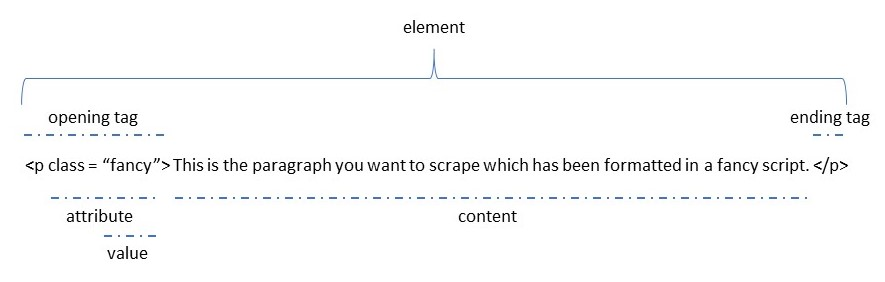
\includegraphics[width=12.29in]{src/images/element_decomp} 

}

\caption{the lingo of an HTML element}\label{fig:unnamed-chunk-24}
\end{figure}

\begin{bonus}
The class attribute is a flexible one. Many web developers use the class
attribute to point to a class name in a style sheet or to access and
manipulate elements with the specific class name with a JavaScript. For
more information of the class attribute, see this
\href{https://www.w3schools.com/html/html_classes.asp}{link}. For more
information on cascading style sheets which are used to decorate HTML
pages, see this \href{https://www.w3schools.com/css/}{link}.
\end{bonus}

\begin{feedback}
Any feedback for this section? Click
\href{https://docs.google.com/forms/d/e/1FAIpQLSePQZ3lIaCIPo9J2owXImHZ_9wBEgTo21A0s-A1ty28u4yfvw/viewform?entry.1684471501=The\%20R\%20Community}{here}
\end{feedback}

\hypertarget{selector-gadgets}{%
\paragraph{Selector Gadgets}\label{selector-gadgets}}

While all web pages are composed of HTML elements, the elements themselves can be structured in complicated ways. Elements are often nested inside one another or make use of elements in other documents. These complicated structures can make scraping data difficult. Thankfully, we can circumvent exploring these complicated structures with the help of selector gadgets.

A \textbf{selector gadget} allows you to determine what css selector you need to extract the information desired from a webpage. These JavaScript bookmarklets allow you to determine where the information you desire belongs within the complicated structure of elements that makeup a webpage. To follow along in Chapter 3, you will need to download one of these gadgets from this \href{https://selectorgadget.com/}{link}. If you use Google Chrome, you can download the bookmark extension directly from this \href{https://selectorgadget.com/}{link}.

If the selector gadget fails us, we can always view the structure of the elements directly by viewing the page source. This can be done by right-clicking on the webpage and selecting `View Page Source'. For Google Chrome, you can also use the keyboard shortcut `CTRL-U'.

\hypertarget{scraping-nfl-data}{%
\subsubsection{Scraping NFL Data}\label{scraping-nfl-data}}

In Chapter \ref{APIs}, we gathered some betting data pertaining to the NFL through a web-API. We may wish to supplement these betting data with data pertaining to NFL teams, players, or even playing conditions. The goal in this subsection is to introduce you to scraping by heeding the advice given in the Chapter \ref{LessonsLearnedFromScraping}. Further examples are given in the supplemental material.

Following our own advice, let's brainstorm. When you think of NFL data, you probably think of \href{https://www.nfl.com/stats}{NFL.com} or \href{https://www.espn.com/nfl/stats}{ESPN}. These sites obviously have reliable data, but the webpages are pretty involved. While the filters, dropdown menus, and graphics lend great experiences for web browsers, they create headaches for web scrapers. After further digging, we will explore \href{https://www.pro-football-reference.com/}{Pro Football Reference}, a reliable archive for football statistics (with a reasonably simple webpage). This is an exhaustive source which boasts team statistics, player statistics, and playing conditions for various seasons. Let's now start small by focusing on team statistics, but further, let's limit our scope to the \href{https://www.pro-football-reference.com/teams/den/2020.htm}{2020 Denver Broncos}. Notice, there are hyperlinks for each \href{https://www.pro-football-reference.com/players/G/GordMe00.htm}{player} documented in any of the categories, as well hyperlinks for each game's \href{https://www.pro-football-reference.com/boxscores/202009140den.htm}{boxscore} where there is information about playing conditions and outcomes. Hence, we have a common thread between team statistics, players, and boxscores. If, for example, we chose to scrape team statistics from one website and player statistics from another website, we may have to worry about a unique identifier (being team) if the websites have different naming conventions.

\hypertarget{html-tables-team-statistics}{%
\paragraph{HTML Tables: Team Statistics}\label{html-tables-team-statistics}}

We'll start with the team statistics for the 2020 Denver Broncos which can be found in a table entitled `Team Stats and Rankings'. We'll need to figure in which element or \textbf{node} the table lives within the underlying HTML. To do this, we will utilize the CSS selector gadget. If we highlight over and click the table with the selector gadget, we will see that the desired table lives in an element called `\#team\_stats'.

\begin{figure}

{\centering 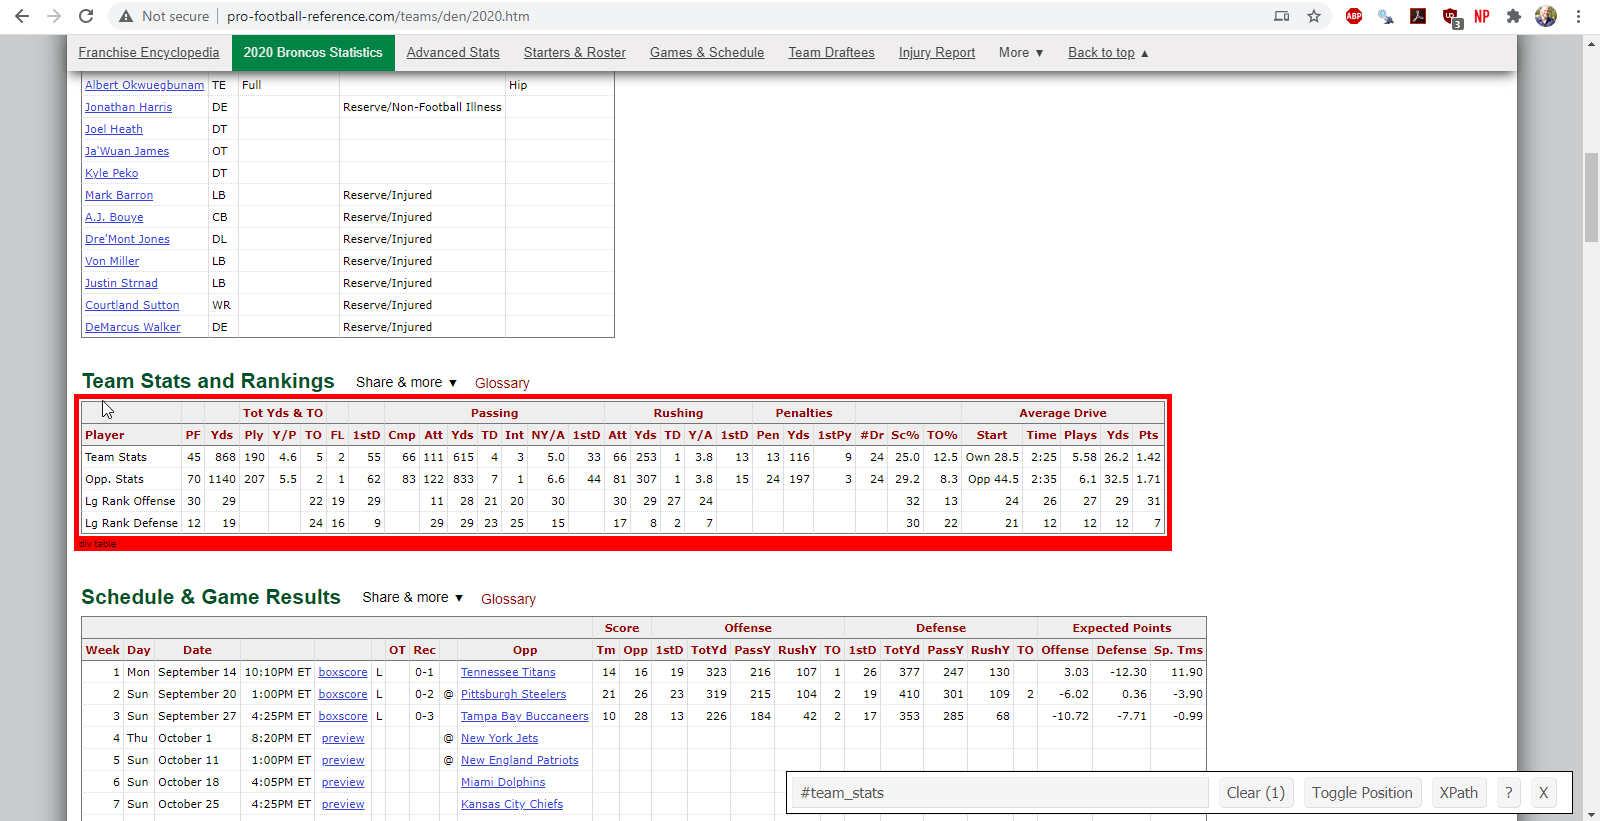
\includegraphics[width=22.22in]{src/images/broncos_selector_gadget} 

}

\caption{finding the team statistics element using the selector gadget}\label{fig:unnamed-chunk-27}
\end{figure}

Alternatively, we could view the page source and search for the table name. I've highlighted the information identified by the selector gadget with the cursor.

\begin{figure}

{\centering 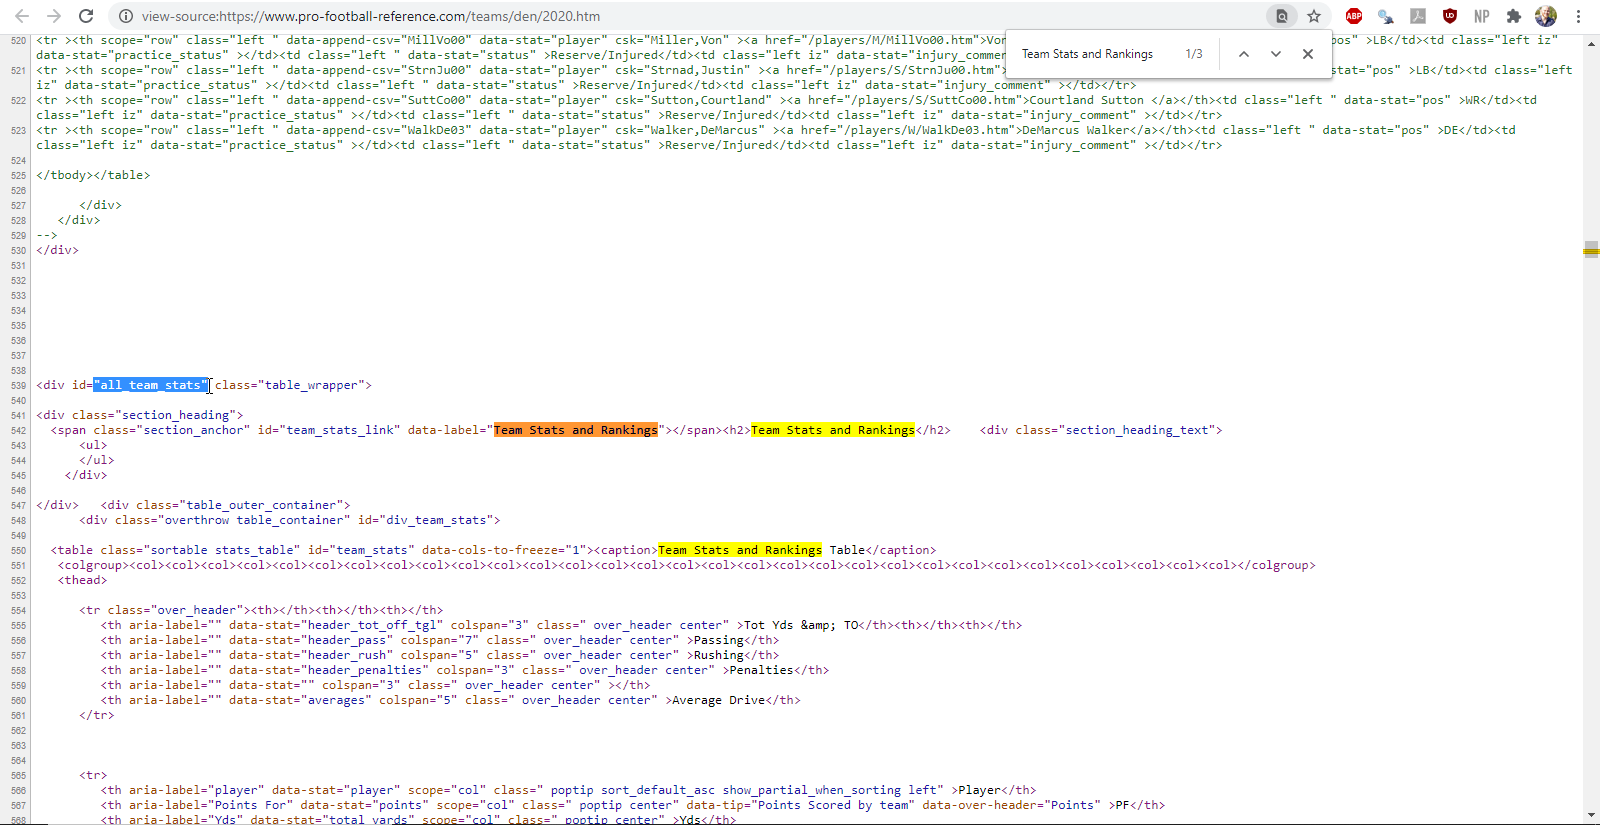
\includegraphics[width=22.22in]{src/images/broncos_page_source} 

}

\caption{finding the team statistics element using the page source}\label{fig:unnamed-chunk-28}
\end{figure}

\begin{caution}
While the selector gadget is always a great first option, it is not
always reliable. There are instances when the selector gadget identifies
a node that is hidden or inaccessible without JavaScript. In these
situations, it is best view the page source directly for more guidance
on how to proceed. Practice with both the selector gadget and the page
source.
\end{caution}

Once we have found the name of the element containing the desired data, we can utilize the \texttt{rvest} package to scrape the table. The general process for scraping an HTML table is

\begin{enumerate}
\def\labelenumi{\arabic{enumi}.}
\tightlist
\item
  Read the HTML identified by the web address.
\item
  Isolate the node containing the data we desire.
\item
  Parse the HTML table.
\item
  Take a look at the data to ensure the columns are appropriate labels.
\end{enumerate}

\begin{Shaded}
\begin{Highlighting}[]
\KeywordTok{library}\NormalTok{(rvest)}
\KeywordTok{library}\NormalTok{(janitor)}

\NormalTok{pfr_url <-}\StringTok{ "https://www.pro-football-reference.com"}
\NormalTok{broncos_url <-}\StringTok{ }\KeywordTok{str_c}\NormalTok{(pfr_url, }\StringTok{'/teams/den/2020.htm'}\NormalTok{)}

\NormalTok{broncos_url }\OperatorTok
\StringTok{  }\CommentTok{# read the HTML}
\StringTok{  }\KeywordTok{read_html}\NormalTok{(.) }\OperatorTok
\StringTok{  }\CommentTok{# isolate the node containing the HTML table}
\StringTok{  }\KeywordTok{html_node}\NormalTok{(., }\DataTypeTok{css =} \StringTok{'#team_conversions'}\NormalTok{) }\OperatorTok
\StringTok{  }\CommentTok{# parse the html table}
\StringTok{  }\KeywordTok{html_table}\NormalTok{(.) }\OperatorTok
\StringTok{  }\CommentTok{# make the first row of the table column headers and clean up column names}
\StringTok{  }\KeywordTok{row_to_names}\NormalTok{(., }\DataTypeTok{row_number =} \DecValTok{1}\NormalTok{) }\OperatorTok
\StringTok{  }\KeywordTok{clean_names}\NormalTok{()}
\end{Highlighting}
\end{Shaded}

\begin{verbatim}
           player x3d_att x3d_conv x3d_percent x4d_att x4d_conv x4d_percent
2      Team Stats      50       19        38.0       4        0         0.0
3      Opp. Stats      63       25        39.7       6        3        50.0
4 Lg Rank Offense                           25                           30
5 Lg Rank Defense                           12                           12
  rz_att rztd rz_pct
2     13    6   46.2
3     13    6   46.2
4                 28
5                  4
\end{verbatim}

While these data need cleaning up before they can be used in practice, we will defer these responsibilities to Chapter \ref{Wrangling}.

\begin{progress}
Take this time to scrape the `Team Conversions' table on your own.
\end{progress}

\begin{feedback}
Any feedback for this section? Click
\href{https://docs.google.com/forms/d/e/1FAIpQLSePQZ3lIaCIPo9J2owXImHZ_9wBEgTo21A0s-A1ty28u4yfvw/viewform?entry.1684471501=The\%20R\%20Community}{here}
\end{feedback}

\hypertarget{ScrapingInTheWild}{%
\section{Scraping in the Wild}\label{ScrapingInTheWild}}

\begin{quote}
``You can have data without information, but you cannot have information without data.'' --- Daniel Keys Moran, Computer Scientist and Author
\end{quote}

In Chapter \ref{AccessingData}, we introduced the idea of rectangular data vs.~non-rectangular data, providing examples for each and demonstrating the process of rectangularization. We outlined how to use a web-API before introducing the concept of web scraping by illustrating the language of the web: HTML. Since webpages can be complicated, scraping can be complicated. In this chapter, we will leverage the Selector Gadget and our knowledge of HTML elements to scrape data from various sources. It is our belief that the only way to teach web scraping is through examples. Each example will become slightly more difficult than the previous.

\hypertarget{LessonsLearnedFromScraping}{%
\subsection{Lessons Learned from Scraping}\label{LessonsLearnedFromScraping}}

Scraping is a necessary evil that requires patience. While some tasks may prove easy, you will quickly find others seem insurmountable. In this section, we will outline a few tips to help you become a web scraper.

\begin{enumerate}
\def\labelenumi{\arabic{enumi}.}
\item
  \textbf{Brainstorm}! Before jumping into your scraping project, ask yourself \emph{what data do I need} and \emph{where can I find it}? If you discover you need data from various sources, \emph{what is the unique identifier}, the link which ties these data together? Taking the time to explore different websites can save you a vast amount of time in the long run. As a general rule, simplistic looking websites are generally easier to scrape and often contain the same information as more complicated websites with several bells and whistles.
\item
  \textbf{Start small}! Sometimes a scraping task can feel daunting, but it is important to \emph{view your project as a war, splitting it up into small battles}. If you are interested in the racial demographics of each of the United States, consider how you can first scrape this information for one state. In this process, don't forget tip 1!
\item
  \textbf{Hyperlinks are your friend}! They can lead to websites with more detailed information or serve as the unique identifier you need between different data sources. Sometimes you won't even need to scrape the hyperlinks to navigate between webpages, making minor adjustments to the web address will sometimes do.
\item
  \textbf{Data is everywhere}! Text color, font, or highlighting may serve as valuable data that you need. If these features exist on the webpage, then they exist within the HTML code which generated the document. Sometimes these features are well hidden or even inaccessible, leading to the last and final tip.
\item
  \textbf{Ready your search engine}! Just like coding in \texttt{R} is an art, web developing is an art. When asking distinct developers to create the same website with the same functionality, the final result may be similar but the underlying HTML code could be drastically different. Why does this matter? You will run into an issue that hasn't been addressed in this text. Thankfully, if you've run into an issue, someone else probably has too. We cannot recommend websites like \href{https://stackoverflow.com/}{Stack Overflow} enough.
\end{enumerate}

\hypertarget{scraping-nfl-data-1}{%
\subsection{Scraping NFL Data}\label{scraping-nfl-data-1}}

In Chapter \ref{AccessingData}, we gathered some betting data pertaining to the NFL through a web-API. We may wish to supplement these betting data with data pertaining to NFL teams, players, or even playing conditions. As we progress through this sub-section, examples will become increasingly problematic or troublesome. The goal in this subsection is to introduce you to scraping by heeding the advice given in the Chapter \ref{LessonsLearnedFromScraping}.

Following our own advice, let's brainstorm. When you think of NFL data, you probably think of \href{https://www.nfl.com/stats}{NFL.com} or \href{https://www.espn.com/nfl/stats}{ESPN}. After further digging, we will explore \href{https://www.pro-football-reference.com/}{Pro Football Reference}, a reliable archive for football statistics (with a reasonably simple webpage). This is an exhaustive source which boasts team statistics, player statistics, and playing conditions for various seasons. Let's now start small by focusing on team statistics, but further, let's limit our scope to the \href{https://www.pro-football-reference.com/teams/den/2020.htm}{2020 Denver Broncos}. Notice, there are hyperlinks for each \href{https://www.pro-football-reference.com/players/G/GordMe00.htm}{player} documented in any of the categories, as well hyperlinks for each game's \href{https://www.pro-football-reference.com/boxscores/202009140den.htm}{boxscore} where there is information about playing conditions and outcomes. Hence, we have a common thread between team statistics, players, and boxscores. If, for example, we chose to scrape team statistics from one website and player statistics from another website, we may have to worry about a unique identifier (being team) if the websites have different naming conventions.

\hypertarget{html-tables-team-statistics-1}{%
\subsubsection{HTML Tables: Team Statistics}\label{html-tables-team-statistics-1}}

We'll start with the team statistics for the 2020 Denver Broncos which can be found in a table entitled `Team Stats and Rankings'. We'll need to figure in which element or \textbf{node} the table lives within the underlying HTML. To do this, we will utilize the CSS selector gadget. If we highlight over and click the table with the selector gadget, we will see that the desired table lives in an element called `\#team\_stats'.

\begin{figure}

{\centering 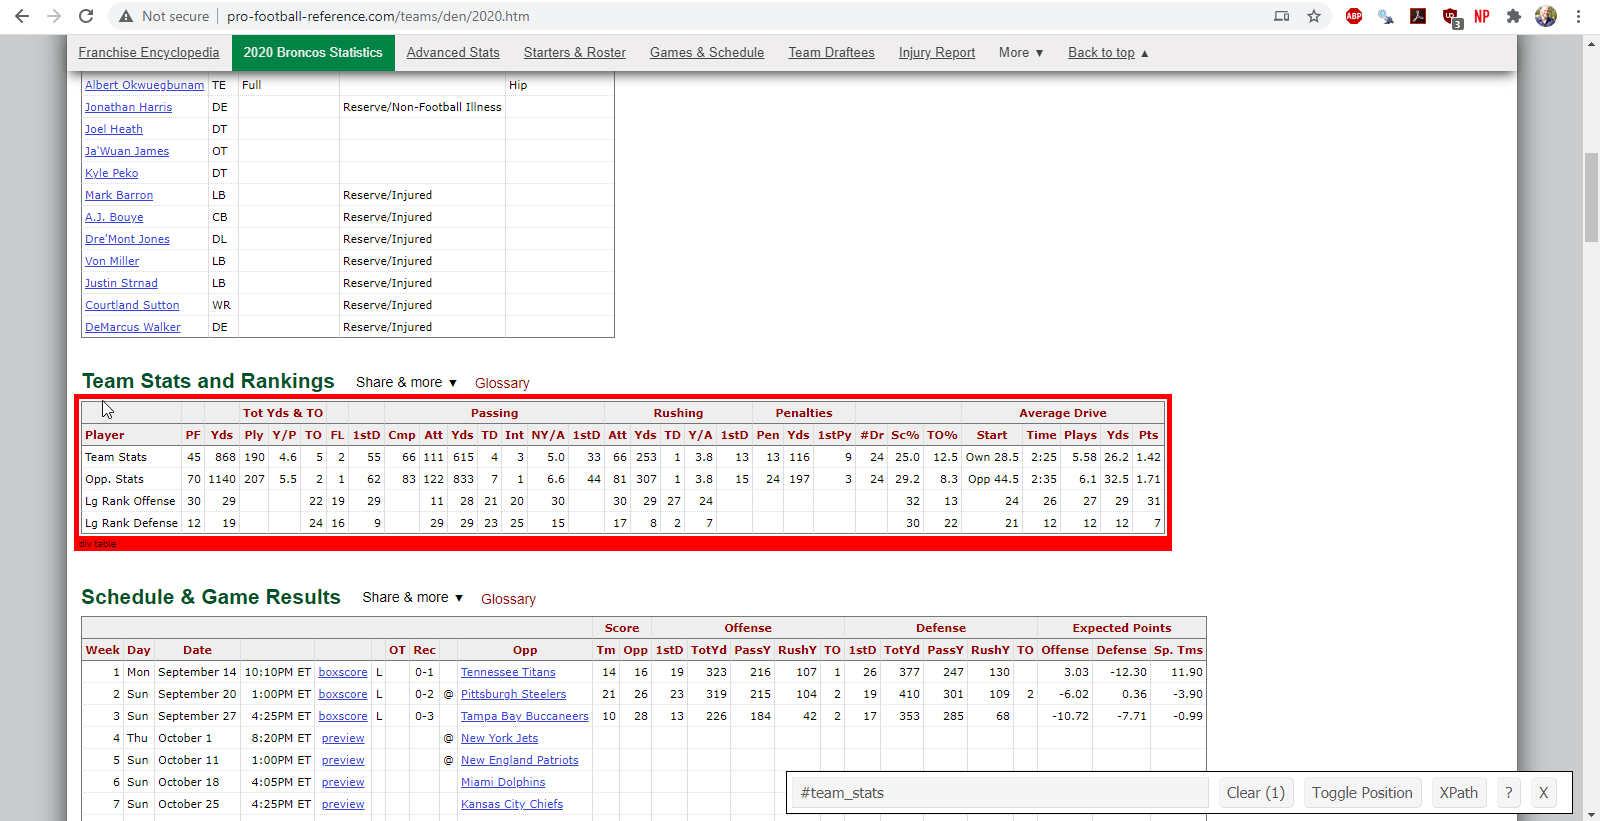
\includegraphics[width=22.22in]{src/images/broncos_selector_gadget} 

}

\caption{finding the team statistics element using the selector gadget}\label{fig:unnamed-chunk-33}
\end{figure}

Alternatively, we could view the page source and search for the table name. I've highlighted the information identified by the selector gadget with the cursor.

\begin{figure}

{\centering 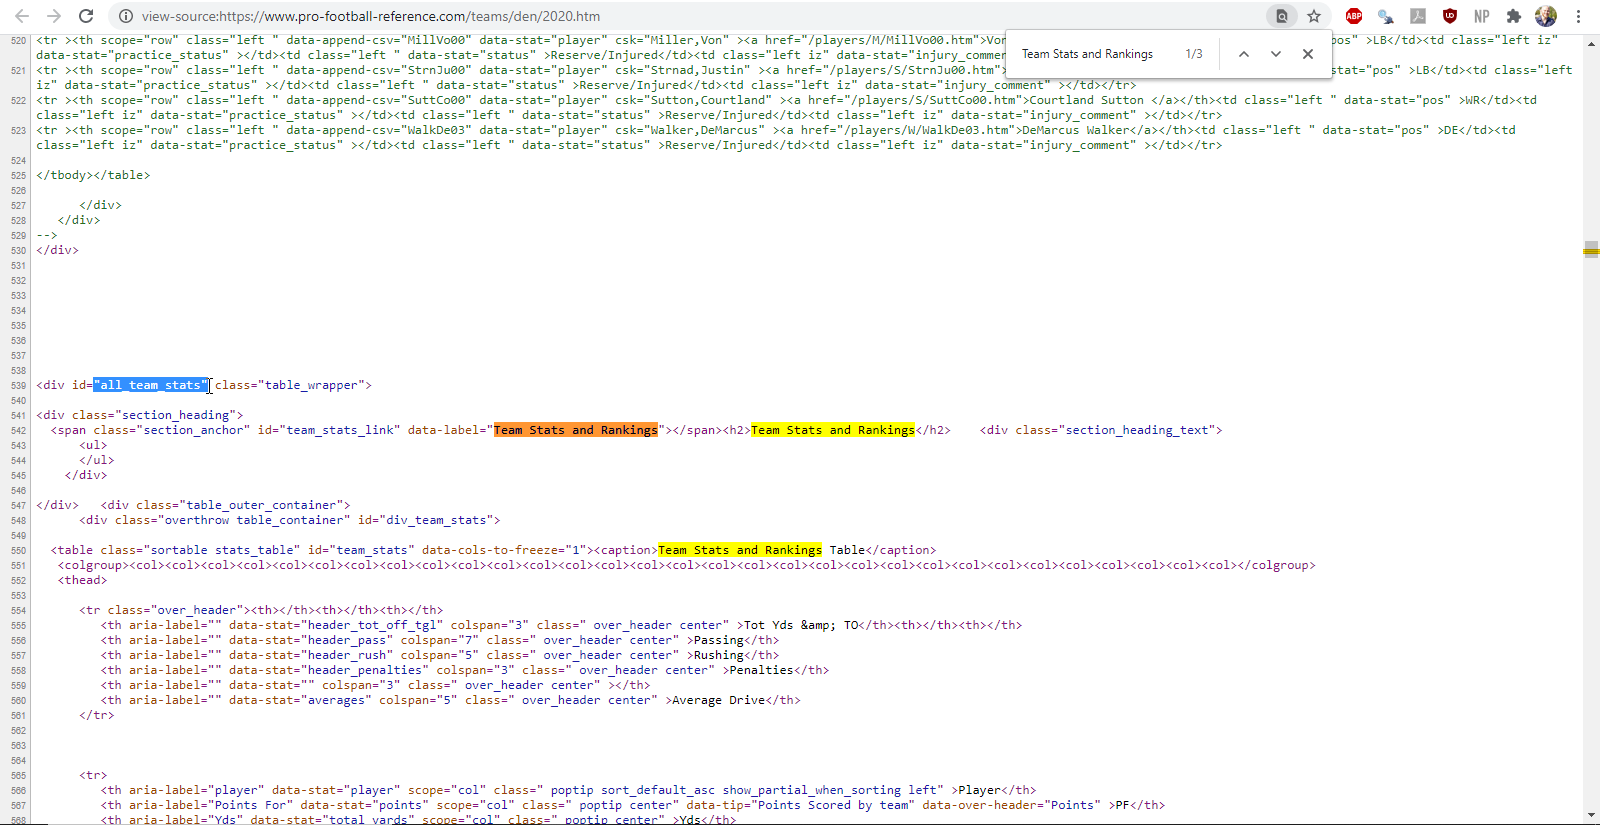
\includegraphics[width=22.22in]{src/images/broncos_page_source} 

}

\caption{finding the team statistics element using the page source}\label{fig:unnamed-chunk-34}
\end{figure}

\begin{caution}
While the selector gadget is always a great first option, it is not
always reliable. There are instances when the selector gadget identifies
a node that is hidden or inaccessible without JavaScript. In these
situations, it is best view the page source directly for more guidance
on how to proceed. Practice with both the selector gadget and the page
source.
\end{caution}

Once we have found the name of the element containing the desired data, we can utilize the \texttt{rvest} package to scrape the table. The general process for scraping an HTML table is

\begin{enumerate}
\def\labelenumi{\arabic{enumi}.}
\tightlist
\item
  Read the HTML identified by the web address.
\item
  Isolate the node containing the data we desire.
\item
  Parse the HTML table.
\item
  Take a look at the data to ensure the columns are appropriate labels.
\end{enumerate}

\begin{Shaded}
\begin{Highlighting}[]
\KeywordTok{library}\NormalTok{(rvest)}
\KeywordTok{library}\NormalTok{(janitor)}

\NormalTok{pfr_url <-}\StringTok{ "https://www.pro-football-reference.com"}
\NormalTok{broncos_url <-}\StringTok{ }\KeywordTok{str_c}\NormalTok{(pfr_url, }\StringTok{'/teams/den/2020.htm'}\NormalTok{)}

\NormalTok{broncos_url }\OperatorTok
\StringTok{  }\CommentTok{# read the HTML}
\StringTok{  }\KeywordTok{read_html}\NormalTok{(.) }\OperatorTok
\StringTok{  }\CommentTok{# isolate the node containing the HTML table}
\StringTok{  }\KeywordTok{html_node}\NormalTok{(., }\DataTypeTok{css =} \StringTok{'#team_conversions'}\NormalTok{) }\OperatorTok
\StringTok{  }\CommentTok{# parse the html table}
\StringTok{  }\KeywordTok{html_table}\NormalTok{(.) }\OperatorTok
\StringTok{  }\CommentTok{# make the first row of the table column headers and clean up column names}
\StringTok{  }\KeywordTok{row_to_names}\NormalTok{(., }\DataTypeTok{row_number =} \DecValTok{1}\NormalTok{) }\OperatorTok
\StringTok{  }\KeywordTok{clean_names}\NormalTok{()}
\end{Highlighting}
\end{Shaded}

\begin{verbatim}
           player x3d_att x3d_conv x3d_percent x4d_att x4d_conv x4d_percent
2      Team Stats      50       19        38.0       4        0         0.0
3      Opp. Stats      63       25        39.7       6        3        50.0
4 Lg Rank Offense                           25                           30
5 Lg Rank Defense                           12                           12
  rz_att rztd rz_pct
2     13    6   46.2
3     13    6   46.2
4                 28
5                  4
\end{verbatim}

While these data need cleaning up before they can be used in practice, we will defer these responsibilities to Chapter \ref{Wrangling}.

\begin{progress}
In the next subsection, we will take a deeper dive into scraping HTML
tables using information attained from attribute values, a common
occurrence in web scraping. Take this time to scrape the `Team
Conversions' table on your own.
\end{progress}

\begin{feedback}
Any feedback for this section? Click
\href{https://docs.google.com/forms/d/e/1FAIpQLSePQZ3lIaCIPo9J2owXImHZ_9wBEgTo21A0s-A1ty28u4yfvw/viewform?entry.1684471501=The\%20R\%20Community}{here}
\end{feedback}

\hypertarget{commented-and-hidden-html-tables-player-statistics}{%
\subsubsection{Commented and Hidden HTML Tables: Player Statistics}\label{commented-and-hidden-html-tables-player-statistics}}

Let's transition to gathering player statistics, particularly for those players who have recorded statistics in the rushing or receiving category. These data are given in the table entitled `Rushing and Receiving'. Let's use the selector gadget to identify the node containing the table and scrape the table according to the previous section.

\begin{Shaded}
\begin{Highlighting}[]
\NormalTok{broncos_url }\OperatorTok
\StringTok{  }\CommentTok{# read the HTML}
\StringTok{  }\KeywordTok{read_html}\NormalTok{(.) }\OperatorTok
\StringTok{  }\CommentTok{# isolate the node containing the HTML table}
\StringTok{  }\KeywordTok{html_node}\NormalTok{(., }\DataTypeTok{css =} \StringTok{'#rushing_and_receiving'}\NormalTok{) }\OperatorTok
\StringTok{  }\CommentTok{# parse the html table}
\StringTok{  }\KeywordTok{html_table}\NormalTok{(.)}
\end{Highlighting}
\end{Shaded}

We get an error stating that the node `\#rushing\_and\_receiving' does not contain an HTML table. In fact, there doesn't appear to be anything in that node at all.

\begin{Shaded}
\begin{Highlighting}[]
\NormalTok{broncos_url }\OperatorTok
\StringTok{  }\CommentTok{# read the HTML}
\StringTok{  }\KeywordTok{read_html}\NormalTok{(.) }\OperatorTok
\StringTok{  }\CommentTok{# isolate the node containing the HTML table}
\StringTok{  }\KeywordTok{html_node}\NormalTok{(., }\DataTypeTok{css =} \StringTok{'#rushing_and_receiving'}\NormalTok{)}
\end{Highlighting}
\end{Shaded}

\begin{verbatim}
{xml_missing}
<NA>
\end{verbatim}

This, of course, is contrary to the selector gadget declaring a node `\#rushing\_and\_receiving' as the one containing the table we desire and directly see on the webpage. Generally when this happens, it means the node containing the information in the table has either been \textbf{commented out} or \textbf{hidden}. A node is commented out when it is contained in a \textbf{comment tag}: \texttt{\textless{}!-\/-\ -\/-\textgreater{}}. For example, if we were to comment out the paragraph element in Chapter \ref{AccessingData}, it would look like this:

\texttt{\textless{}!-\/-\ \textless{}p\ class\ =\ "fancy"\textgreater{}\ This\ is\ the\ paragraph\ you\ want\ to\ scrape\ which\ has\ been\ formatted\ in\ a\ fancy\ script.\ \textless{}/p\textgreater{}\ -\/-\textgreater{}}.

When a node is commented out, it exists in the HTML, but it cannot be accessed until we step into the comment tag. Otherwise said, we can't bypass the comment node. If you would like to scrape information contained with a comment tag, the general strategy is

\begin{enumerate}
\def\labelenumi{\arabic{enumi}.}
\tightlist
\item
  Read the HTML identified by the web address.
\item
  Isolate the node containing the comment tag. Inside the comment tag are the data we desire.
\item
  Isolate the comment tag.
\item
  Convert the content to HTML.
\item
  Isolate the node containing the table.
\item
  Parse the HTML table.
\item
  Take a look at the data to ensure the columns are appropriate labels.
\end{enumerate}

\begin{Shaded}
\begin{Highlighting}[]
\NormalTok{broncos_url }\OperatorTok
\StringTok{  }\KeywordTok{read_html}\NormalTok{() }\OperatorTok
\StringTok{  }\KeywordTok{html_node}\NormalTok{(., }\DataTypeTok{css =} \StringTok{'#all_rushing_and_receiving'}\NormalTok{) }\OperatorTok
\StringTok{  }\KeywordTok{html_nodes}\NormalTok{(., }\DataTypeTok{xpath =} \StringTok{'comment()'}\NormalTok{) }\OperatorTok
\StringTok{  }\KeywordTok{html_text}\NormalTok{() }\OperatorTok
\StringTok{  }\KeywordTok{read_html}\NormalTok{() }\OperatorTok
\StringTok{  }\KeywordTok{html_node}\NormalTok{(., }\StringTok{'table'}\NormalTok{) }\OperatorTok
\StringTok{  }\KeywordTok{html_table}\NormalTok{() }\OperatorTok
\StringTok{  }\KeywordTok{set_names}\NormalTok{(., }\KeywordTok{str_c}\NormalTok{(}\KeywordTok{names}\NormalTok{(.), .[}\DecValTok{1}\NormalTok{,], }\DataTypeTok{sep =} \StringTok{'_'}\NormalTok{)) }\OperatorTok
\StringTok{  }\KeywordTok{clean_names}\NormalTok{() }\OperatorTok
\StringTok{  }\KeywordTok{slice}\NormalTok{(., }\DecValTok{-1}\NormalTok{)}
\end{Highlighting}
\end{Shaded}

\begin{verbatim}
   no           player  age pos games_g games_gs rushing_att rushing_yds
1  25    Melvin Gordon   27  rb       4        4          65         281
2  28    Royce Freeman   24           4        0           9          30
3  30  Phillip Lindsay   26  rb       1        1           7          24
4   9     Jeff Driskel   27  qb       3        1           6          28
5   4     Brett Rypien   24  qb       2        1           5          -5
6   3        Drew Lock   24  qb       2        2           3           5
7  13        KJ Hamler   21  wr       3        2           2           7
8   6       Sam Martin   30   p       4        0           1           0
9  87        Noah Fant   23  te       4        4           0           0
10 81      Tim Patrick   27  wr       4        4           0           0
11 10      Jerry Jeudy   21  wr       4        2           0           0
12 17 DaeSean Hamilton   25  wr       4        1           0           0
13 14 Courtland Sutton   25  wr       1        1           0           0
14 80        Jake Butt   25           4        0           0           0
15 88     Nick Vannett   27  te       3        1           0           0
16 16  Tyrie Cleveland   23           3        0           0           0
17 11  Diontae Spencer   28           4        0           0           0
18          Team Total 25.5           4                   98         370
19           Opp Total                4                  105         436
   rushing_td rushing_lng rushing_y_a rushing_y_g rushing_a_g receiving_tgt
1           3          43         4.3        70.3        16.3            15
2           0          13         3.3         7.5         2.3             5
3           0          10         3.4        24.0         7.0             1
4           0           9         4.7         9.3         2.0              
5           0          -1        -1.0        -2.5         2.5              
6           0           3         1.7         2.5         1.5              
7           0           9         3.5         2.3         0.7            12
8           0           0         0.0         0.0         0.3              
9           0           0                     0.0         0.0            27
10          0           0                     0.0         0.0            21
11          0           0                     0.0         0.0            28
12          0           0                     0.0         0.0             9
13          0           0                     0.0         0.0             6
14          0           0                     0.0         0.0             4
15          0           0                     0.0         0.0             6
16          0           0                     0.0         0.0             1
17          0           0                     0.0         0.0             1
18          3          43         3.8        92.5        24.5           136
19          2                     4.2       109.0        26.3              
   receiving_rec receiving_yds receiving_y_r receiving_td receiving_lng
1             11            45           4.1            1            16
2              5            49           9.8            0            28
3              1            11          11.0            0            11
4                                                                      
5                                                                      
6                                                                      
7              6            78          13.0            0            18
8                                                                      
9             19           219          11.5            2            31
10            16           209          13.1            2            40
11            15           234          15.6            1            48
12             3            32          10.7            0            18
13             3            66          22.0            0            45
14             2             5           2.5            0             5
15             2             1           0.5            0             7
16             1             7           7.0            0             7
17             1             7           7.0            0             7
18            85           963          11.3            6            48
19           108          1025           9.5            7              
   receiving_r_g receiving_y_g receiving_ctch_percent receiving_y_tgt
1            2.8          11.3                  73.3%             3.0
2            1.3          12.3                 100.0%             9.8
3            1.0          11.0                 100.0%            11.0
4                                                                    
5                                                                    
6                                                                    
7            2.0          26.0                  50.0%             6.5
8                                                                    
9            4.8          54.8                  70.4%             8.1
10           4.0          52.3                  76.2%            10.0
11           3.8          58.5                  53.6%             8.4
12           0.8           8.0                  33.3%             3.6
13           3.0          66.0                  50.0%            11.0
14           0.5           1.3                  50.0%             1.3
15           0.7           0.3                  33.3%             0.2
16           0.3           2.3                 100.0%             7.0
17           0.3           1.8                 100.0%             7.0
18          21.3         240.8                  62.5%                
19          27.0         256.3                                       
   total_yds_touch total_yds_y_tch total_yds_y_scm rrtd fmb
1               76             4.3             326    4   1
2               14             5.6              79    0   0
3                8             4.4              35    0   0
4                6             4.7              28    0   0
5                5            -1.0              -5    0   1
6                3             1.7               5    0   3
7                8            10.6              85    0   0
8                1             0.0               0    0   1
9               19            11.5             219    2   0
10              16            13.1             209    2   0
11              15            15.6             234    1   1
12               3            10.7              32    0   0
13               3            22.0              66    0   0
14               2             2.5               5    0   0
15               2             0.5               1    0   0
16               1             7.0               7    0   0
17               1             7.0               7    0   0
18             183             7.3            1333    9   7
19                                            1461    9   3
\end{verbatim}

\hypertarget{attributes-player-statistics-by-game}{%
\subsubsection{Attributes: Player Statistics by Game}\label{attributes-player-statistics-by-game}}

Suppose now that we wish to scrape the same player statistics, but rather than get the aggregated total, we want the players' statistics by game. Within the Rushing and Receiving table scraped in the previous example, there are hyperlinks for each player. When you click on this hyperlink, you will find the player's statistics for each game played. These are the data we desire. We want rushing and receiving statistics for each player on each team for a variety of years. Using the lessons learned in Chapter \ref{LessonsLearnedFromScraping}, we have brainstormed the problem and have a road map to the solution. We will first scrape the hyperlink attribute to get the web address associated with each player for a given team. Within each of these web addresses, we will scrape the game by game statistics before iterating over each team in the NFL. After this, we can repeat the procedure for a variety of years. This is, of course, a big job, so let's scale down the problem to one player: Melvin Gordon III, running back. To do this, we will:

\begin{enumerate}
\def\labelenumi{\arabic{enumi}.}
\tightlist
\item
  Get the web addresses associated with each player in the Rushing and Receiving table, before isolating the address associated with Melvin Gordon's rushing and receiving statistics.
\item
  Read the HTML identified by the web address.
\item
  Isolate the node containing the data we desire.
\item
  Parse the HTML table.
\item
  Take a look at the data to ensure the columns are appropriate labels.
\end{enumerate}

Let's figure out where the hyperlinks exist within the HTML code. To do this, I will look at the page source and search for Melvin Gordon. We find that the web address corresponding to his game by game player statistics exist in the hidden HTML table that we scraped in the previous example. In particular, they are the \texttt{href} attribute to a node entitled \texttt{a} which is embedded within the hidden HTML table. Phew. Let's consider how we can scrape these web addresses step by step:

1.1 Isolate the hidden HTML table, similar to the previous example.
1.2 Isolate nodes with tag \texttt{a}.
1.3 Extract the \texttt{href} attribute from these nodes.

Steps 1.1 and 1.2 should be familiar from previous examples, but step 1.3 requires a new function within \texttt{rvest} called \texttt{html\_attr}. Let's see how to do this in \texttt{R}.

\begin{figure}

{\centering 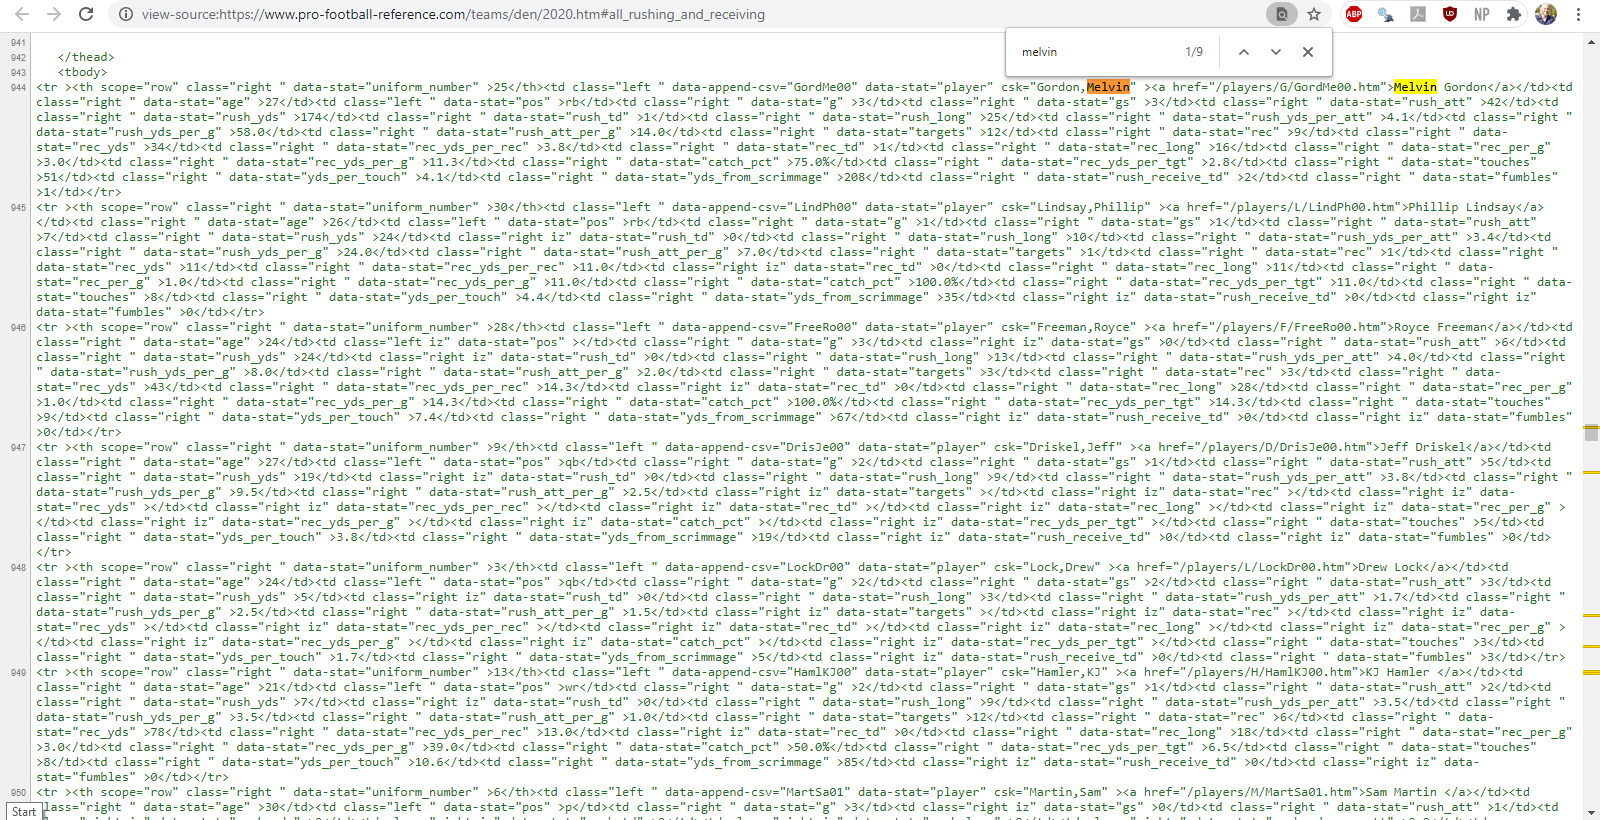
\includegraphics[width=22.22in]{src/images/broncos_gordon_page_source} 

}

\caption{finding the element containing the web address cooresponding to Melvin Gordon III game by game player statistics using the page source}\label{fig:unnamed-chunk-42}
\end{figure}

\begin{Shaded}
\begin{Highlighting}[]
\NormalTok{player_urls <-}\StringTok{ }\NormalTok{broncos_url }\OperatorTok
\StringTok{  }\KeywordTok{read_html}\NormalTok{() }\OperatorTok
\StringTok{  }\KeywordTok{html_node}\NormalTok{(., }\DataTypeTok{css =} \StringTok{'#all_rushing_and_receiving'}\NormalTok{) }\OperatorTok
\StringTok{  }\KeywordTok{html_nodes}\NormalTok{(., }\DataTypeTok{xpath =} \StringTok{'comment()'}\NormalTok{) }\OperatorTok
\StringTok{  }\KeywordTok{html_text}\NormalTok{() }\OperatorTok
\StringTok{  }\KeywordTok{read_html}\NormalTok{() }\OperatorTok
\StringTok{  }\KeywordTok{html_nodes}\NormalTok{(., }\StringTok{'table'}\NormalTok{) }\OperatorTok
\StringTok{  }\KeywordTok{html_nodes}\NormalTok{(., }\StringTok{'a'}\NormalTok{) }\OperatorTok
\StringTok{  }\KeywordTok{html_attr}\NormalTok{(., }\StringTok{'href'}\NormalTok{) }\OperatorTok
\StringTok{  }\KeywordTok{str_c}\NormalTok{(pfr_url, .)}
\NormalTok{player_urls}
\end{Highlighting}
\end{Shaded}

\begin{verbatim}
 [1] "https://www.pro-football-reference.com/players/G/GordMe00.htm"
 [2] "https://www.pro-football-reference.com/players/F/FreeRo00.htm"
 [3] "https://www.pro-football-reference.com/players/L/LindPh00.htm"
 [4] "https://www.pro-football-reference.com/players/D/DrisJe00.htm"
 [5] "https://www.pro-football-reference.com/players/R/RypiBr00.htm"
 [6] "https://www.pro-football-reference.com/players/L/LockDr00.htm"
 [7] "https://www.pro-football-reference.com/players/H/HamlKJ00.htm"
 [8] "https://www.pro-football-reference.com/players/M/MartSa01.htm"
 [9] "https://www.pro-football-reference.com/players/F/FantNo00.htm"
[10] "https://www.pro-football-reference.com/players/P/PatrTi00.htm"
[11] "https://www.pro-football-reference.com/players/J/JeudJe00.htm"
[12] "https://www.pro-football-reference.com/players/H/HamiDa01.htm"
[13] "https://www.pro-football-reference.com/players/S/SuttCo00.htm"
[14] "https://www.pro-football-reference.com/players/B/ButtJa00.htm"
[15] "https://www.pro-football-reference.com/players/V/VannNi00.htm"
[16] "https://www.pro-football-reference.com/players/C/ClevTy00.htm"
[17] "https://www.pro-football-reference.com/players/S/SpenDi00.htm"
\end{verbatim}

Since the web addresses are given as an extension to the Pro Football Reference homepage, we will need to concatenate the strings with \texttt{str\_c()} before saving the result for future use. Now, lets continue to step two in our excursion to get Melvin Gordon's game by game statistics.

\begin{Shaded}
\begin{Highlighting}[]
\NormalTok{player_urls[}\DecValTok{1}\NormalTok{] }\OperatorTok
\StringTok{  }\KeywordTok{read_html}\NormalTok{() }\OperatorTok
\StringTok{  }\KeywordTok{html_node}\NormalTok{(., }\DataTypeTok{css =} \StringTok{'#all_stats'}\NormalTok{) }\OperatorTok
\StringTok{  }\KeywordTok{html_node}\NormalTok{(., }\StringTok{'table'}\NormalTok{) }\OperatorTok
\StringTok{  }\KeywordTok{html_table}\NormalTok{(., }\DataTypeTok{fill =} \OtherTok{TRUE}\NormalTok{) }\OperatorTok
\StringTok{  }\KeywordTok{set_names}\NormalTok{(., }\KeywordTok{str_c}\NormalTok{(}\KeywordTok{names}\NormalTok{(.), .[}\DecValTok{1}\NormalTok{,], }\DataTypeTok{sep =} \StringTok{'_'}\NormalTok{)) }\OperatorTok
\StringTok{  }\KeywordTok{clean_names}\NormalTok{() }\OperatorTok
\StringTok{  }\KeywordTok{slice}\NormalTok{(., }\DecValTok{-1}\NormalTok{)}
\end{Highlighting}
\end{Shaded}

\begin{verbatim}
                                                                                         date
1                                                                                  2020-09-14
2                                                                                  2020-09-20
3                                                                                  2020-09-27
4                                                                                  2020-10-01
5                                                              Upcoming Games · Bye in Week 8
6                                                                                  2020-10-12
7                                                                                  2020-10-18
8                                                                                  2020-10-25
9 Broncos 2020 Stats and Schedule · Melvin Gordon Splits · Melvin Gordon Gamelogs · Penalties
                                                                                         week
1                                                                                           1
2                                                                                           2
3                                                                                           3
4                                                                                           4
5                                                              Upcoming Games · Bye in Week 8
6                                                                                           5
7                                                                                           6
8                                                                                           7
9 Broncos 2020 Stats and Schedule · Melvin Gordon Splits · Melvin Gordon Gamelogs · Penalties
                                                                                           tm
1                                                                                         DEN
2                                                                                         DEN
3                                                                                         DEN
4                                                                                         DEN
5                                                              Upcoming Games · Bye in Week 8
6                                                                                         DEN
7                                                                                         DEN
8                                                                                         DEN
9 Broncos 2020 Stats and Schedule · Melvin Gordon Splits · Melvin Gordon Gamelogs · Penalties
                                                                                            x
1                                                                                            
2                                                                                           @
3                                                                                            
4                                                                                           @
5                                                              Upcoming Games · Bye in Week 8
6                                                                                           @
7                                                                                            
8                                                                                            
9 Broncos 2020 Stats and Schedule · Melvin Gordon Splits · Melvin Gordon Gamelogs · Penalties
                                                                                          opp
1                                                                                         TEN
2                                                                                         PIT
3                                                                                         TAM
4                                                                                         NYJ
5                                                              Upcoming Games · Bye in Week 8
6                                                                                         NWE
7                                                                                         MIA
8                                                                                         KAN
9 Broncos 2020 Stats and Schedule · Melvin Gordon Splits · Melvin Gordon Gamelogs · Penalties
                                                                                       result
1                                                                                     L 14-16
2                                                                                     L 21-26
3                                                                                     L 10-28
4                                                                                     W 37-28
5                                                              Upcoming Games · Bye in Week 8
6                Preview · Stats for 1 game vs. Patriots ·   14 rush, 132 yds, 1 TD (in 2017)
7 Preview · Stats for 3 games vs. Dolphins ·  Avg. 16.0 rush, 41.3 yds, 0.3 TD (Last in 2017)
8   Preview · Stats for 8 games vs. Chiefs ·  Avg. 15.3 rush, 58.1 yds, 0.6 TD (Last in 2019)
9 Broncos 2020 Stats and Schedule · Melvin Gordon Splits · Melvin Gordon Gamelogs · Penalties
                                                                                           gs
1                                                                                           *
2                                                                                           *
3                                                                                           *
4                                                                                           *
5                                                              Upcoming Games · Bye in Week 8
6                Preview · Stats for 1 game vs. Patriots ·   14 rush, 132 yds, 1 TD (in 2017)
7 Preview · Stats for 3 games vs. Dolphins ·  Avg. 16.0 rush, 41.3 yds, 0.3 TD (Last in 2017)
8   Preview · Stats for 8 games vs. Chiefs ·  Avg. 15.3 rush, 58.1 yds, 0.6 TD (Last in 2019)
9 Broncos 2020 Stats and Schedule · Melvin Gordon Splits · Melvin Gordon Gamelogs · Penalties
                                                                                 rushing_rush
1                                                                                          15
2                                                                                          19
3                                                                                           8
4                                                                                          23
5                                                              Upcoming Games · Bye in Week 8
6                Preview · Stats for 1 game vs. Patriots ·   14 rush, 132 yds, 1 TD (in 2017)
7 Preview · Stats for 3 games vs. Dolphins ·  Avg. 16.0 rush, 41.3 yds, 0.3 TD (Last in 2017)
8   Preview · Stats for 8 games vs. Chiefs ·  Avg. 15.3 rush, 58.1 yds, 0.6 TD (Last in 2019)
9 Broncos 2020 Stats and Schedule · Melvin Gordon Splits · Melvin Gordon Gamelogs · Penalties
                                                                                  rushing_yds
1                                                                                          78
2                                                                                          70
3                                                                                          26
4                                                                                         107
5                                                              Upcoming Games · Bye in Week 8
6                Preview · Stats for 1 game vs. Patriots ·   14 rush, 132 yds, 1 TD (in 2017)
7 Preview · Stats for 3 games vs. Dolphins ·  Avg. 16.0 rush, 41.3 yds, 0.3 TD (Last in 2017)
8   Preview · Stats for 8 games vs. Chiefs ·  Avg. 15.3 rush, 58.1 yds, 0.6 TD (Last in 2019)
9 Broncos 2020 Stats and Schedule · Melvin Gordon Splits · Melvin Gordon Gamelogs · Penalties
                                                                                  rushing_y_a
1                                                                                        5.20
2                                                                                        3.68
3                                                                                        3.25
4                                                                                        4.65
5                                                              Upcoming Games · Bye in Week 8
6                Preview · Stats for 1 game vs. Patriots ·   14 rush, 132 yds, 1 TD (in 2017)
7 Preview · Stats for 3 games vs. Dolphins ·  Avg. 16.0 rush, 41.3 yds, 0.3 TD (Last in 2017)
8   Preview · Stats for 8 games vs. Chiefs ·  Avg. 15.3 rush, 58.1 yds, 0.6 TD (Last in 2019)
9 Broncos 2020 Stats and Schedule · Melvin Gordon Splits · Melvin Gordon Gamelogs · Penalties
                                                                                   rushing_td
1                                                                                           1
2                                                                                           0
3                                                                                           0
4                                                                                           2
5                                                              Upcoming Games · Bye in Week 8
6                Preview · Stats for 1 game vs. Patriots ·   14 rush, 132 yds, 1 TD (in 2017)
7 Preview · Stats for 3 games vs. Dolphins ·  Avg. 16.0 rush, 41.3 yds, 0.3 TD (Last in 2017)
8   Preview · Stats for 8 games vs. Chiefs ·  Avg. 15.3 rush, 58.1 yds, 0.6 TD (Last in 2019)
9 Broncos 2020 Stats and Schedule · Melvin Gordon Splits · Melvin Gordon Gamelogs · Penalties
                                                                                receiving_tgt
1                                                                                           3
2                                                                                           3
3                                                                                           6
4                                                                                           3
5                                                              Upcoming Games · Bye in Week 8
6                Preview · Stats for 1 game vs. Patriots ·   14 rush, 132 yds, 1 TD (in 2017)
7 Preview · Stats for 3 games vs. Dolphins ·  Avg. 16.0 rush, 41.3 yds, 0.3 TD (Last in 2017)
8   Preview · Stats for 8 games vs. Chiefs ·  Avg. 15.3 rush, 58.1 yds, 0.6 TD (Last in 2019)
9 Broncos 2020 Stats and Schedule · Melvin Gordon Splits · Melvin Gordon Gamelogs · Penalties
                                                                                receiving_rec
1                                                                                           3
2                                                                                           2
3                                                                                           4
4                                                                                           2
5                                                              Upcoming Games · Bye in Week 8
6                Preview · Stats for 1 game vs. Patriots ·   14 rush, 132 yds, 1 TD (in 2017)
7 Preview · Stats for 3 games vs. Dolphins ·  Avg. 16.0 rush, 41.3 yds, 0.3 TD (Last in 2017)
8   Preview · Stats for 8 games vs. Chiefs ·  Avg. 15.3 rush, 58.1 yds, 0.6 TD (Last in 2019)
9 Broncos 2020 Stats and Schedule · Melvin Gordon Splits · Melvin Gordon Gamelogs · Penalties
                                                                                receiving_yds
1                                                                                           8
2                                                                                          14
3                                                                                          12
4                                                                                          11
5                                                              Upcoming Games · Bye in Week 8
6                Preview · Stats for 1 game vs. Patriots ·   14 rush, 132 yds, 1 TD (in 2017)
7 Preview · Stats for 3 games vs. Dolphins ·  Avg. 16.0 rush, 41.3 yds, 0.3 TD (Last in 2017)
8   Preview · Stats for 8 games vs. Chiefs ·  Avg. 15.3 rush, 58.1 yds, 0.6 TD (Last in 2019)
9 Broncos 2020 Stats and Schedule · Melvin Gordon Splits · Melvin Gordon Gamelogs · Penalties
                                                                                receiving_y_r
1                                                                                        2.67
2                                                                                        7.00
3                                                                                        3.00
4                                                                                        5.50
5                                                              Upcoming Games · Bye in Week 8
6                Preview · Stats for 1 game vs. Patriots ·   14 rush, 132 yds, 1 TD (in 2017)
7 Preview · Stats for 3 games vs. Dolphins ·  Avg. 16.0 rush, 41.3 yds, 0.3 TD (Last in 2017)
8   Preview · Stats for 8 games vs. Chiefs ·  Avg. 15.3 rush, 58.1 yds, 0.6 TD (Last in 2019)
9 Broncos 2020 Stats and Schedule · Melvin Gordon Splits · Melvin Gordon Gamelogs · Penalties
                                                                                 receiving_td
1                                                                                           0
2                                                                                           1
3                                                                                           0
4                                                                                           0
5                                                              Upcoming Games · Bye in Week 8
6                Preview · Stats for 1 game vs. Patriots ·   14 rush, 132 yds, 1 TD (in 2017)
7 Preview · Stats for 3 games vs. Dolphins ·  Avg. 16.0 rush, 41.3 yds, 0.3 TD (Last in 2017)
8   Preview · Stats for 8 games vs. Chiefs ·  Avg. 15.3 rush, 58.1 yds, 0.6 TD (Last in 2019)
9 Broncos 2020 Stats and Schedule · Melvin Gordon Splits · Melvin Gordon Gamelogs · Penalties
                                                                       receiving_ctch_percent
1                                                                                      100.0%
2                                                                                       66.7%
3                                                                                       66.7%
4                                                                                       66.7%
5                                                              Upcoming Games · Bye in Week 8
6                Preview · Stats for 1 game vs. Patriots ·   14 rush, 132 yds, 1 TD (in 2017)
7 Preview · Stats for 3 games vs. Dolphins ·  Avg. 16.0 rush, 41.3 yds, 0.3 TD (Last in 2017)
8   Preview · Stats for 8 games vs. Chiefs ·  Avg. 15.3 rush, 58.1 yds, 0.6 TD (Last in 2019)
9 Broncos 2020 Stats and Schedule · Melvin Gordon Splits · Melvin Gordon Gamelogs · Penalties
                                                                              receiving_y_tgt
1                                                                                        2.67
2                                                                                        4.67
3                                                                                        2.00
4                                                                                        3.67
5                                                              Upcoming Games · Bye in Week 8
6                Preview · Stats for 1 game vs. Patriots ·   14 rush, 132 yds, 1 TD (in 2017)
7 Preview · Stats for 3 games vs. Dolphins ·  Avg. 16.0 rush, 41.3 yds, 0.3 TD (Last in 2017)
8   Preview · Stats for 8 games vs. Chiefs ·  Avg. 15.3 rush, 58.1 yds, 0.6 TD (Last in 2019)
9 Broncos 2020 Stats and Schedule · Melvin Gordon Splits · Melvin Gordon Gamelogs · Penalties
                                                                                           td
1                                                                                           1
2                                                                                           1
3                                                                                           0
4                                                                                           2
5                                                              Upcoming Games · Bye in Week 8
6                Preview · Stats for 1 game vs. Patriots ·   14 rush, 132 yds, 1 TD (in 2017)
7 Preview · Stats for 3 games vs. Dolphins ·  Avg. 16.0 rush, 41.3 yds, 0.3 TD (Last in 2017)
8   Preview · Stats for 8 games vs. Chiefs ·  Avg. 15.3 rush, 58.1 yds, 0.6 TD (Last in 2019)
9 Broncos 2020 Stats and Schedule · Melvin Gordon Splits · Melvin Gordon Gamelogs · Penalties
                                                                                  fumbles_fmb
1                                                                                           1
2                                                                                           0
3                                                                                           0
4                                                                                           0
5                                                              Upcoming Games · Bye in Week 8
6                Preview · Stats for 1 game vs. Patriots ·   14 rush, 132 yds, 1 TD (in 2017)
7 Preview · Stats for 3 games vs. Dolphins ·  Avg. 16.0 rush, 41.3 yds, 0.3 TD (Last in 2017)
8   Preview · Stats for 8 games vs. Chiefs ·  Avg. 15.3 rush, 58.1 yds, 0.6 TD (Last in 2019)
9 Broncos 2020 Stats and Schedule · Melvin Gordon Splits · Melvin Gordon Gamelogs · Penalties
                                                                                   fumbles_fl
1                                                                                           1
2                                                                                           0
3                                                                                           0
4                                                                                           0
5                                                              Upcoming Games · Bye in Week 8
6                Preview · Stats for 1 game vs. Patriots ·   14 rush, 132 yds, 1 TD (in 2017)
7 Preview · Stats for 3 games vs. Dolphins ·  Avg. 16.0 rush, 41.3 yds, 0.3 TD (Last in 2017)
8   Preview · Stats for 8 games vs. Chiefs ·  Avg. 15.3 rush, 58.1 yds, 0.6 TD (Last in 2019)
9 Broncos 2020 Stats and Schedule · Melvin Gordon Splits · Melvin Gordon Gamelogs · Penalties
                                                                                   fumbles_ff
1                                                                                           0
2                                                                                           0
3                                                                                           0
4                                                                                           0
5                                                              Upcoming Games · Bye in Week 8
6                Preview · Stats for 1 game vs. Patriots ·   14 rush, 132 yds, 1 TD (in 2017)
7 Preview · Stats for 3 games vs. Dolphins ·  Avg. 16.0 rush, 41.3 yds, 0.3 TD (Last in 2017)
8   Preview · Stats for 8 games vs. Chiefs ·  Avg. 15.3 rush, 58.1 yds, 0.6 TD (Last in 2019)
9 Broncos 2020 Stats and Schedule · Melvin Gordon Splits · Melvin Gordon Gamelogs · Penalties
                                                                                   fumbles_fr
1                                                                                           0
2                                                                                           0
3                                                                                           0
4                                                                                           0
5                                                              Upcoming Games · Bye in Week 8
6                Preview · Stats for 1 game vs. Patriots ·   14 rush, 132 yds, 1 TD (in 2017)
7 Preview · Stats for 3 games vs. Dolphins ·  Avg. 16.0 rush, 41.3 yds, 0.3 TD (Last in 2017)
8   Preview · Stats for 8 games vs. Chiefs ·  Avg. 15.3 rush, 58.1 yds, 0.6 TD (Last in 2019)
9 Broncos 2020 Stats and Schedule · Melvin Gordon Splits · Melvin Gordon Gamelogs · Penalties
                                                                                  fumbles_yds
1                                                                                           0
2                                                                                           0
3                                                                                           0
4                                                                                           0
5                                                              Upcoming Games · Bye in Week 8
6                Preview · Stats for 1 game vs. Patriots ·   14 rush, 132 yds, 1 TD (in 2017)
7 Preview · Stats for 3 games vs. Dolphins ·  Avg. 16.0 rush, 41.3 yds, 0.3 TD (Last in 2017)
8   Preview · Stats for 8 games vs. Chiefs ·  Avg. 15.3 rush, 58.1 yds, 0.6 TD (Last in 2019)
9 Broncos 2020 Stats and Schedule · Melvin Gordon Splits · Melvin Gordon Gamelogs · Penalties
                                                                                   fumbles_td
1                                                                                           0
2                                                                                           0
3                                                                                           0
4                                                                                           0
5                                                              Upcoming Games · Bye in Week 8
6                Preview · Stats for 1 game vs. Patriots ·   14 rush, 132 yds, 1 TD (in 2017)
7 Preview · Stats for 3 games vs. Dolphins ·  Avg. 16.0 rush, 41.3 yds, 0.3 TD (Last in 2017)
8   Preview · Stats for 8 games vs. Chiefs ·  Avg. 15.3 rush, 58.1 yds, 0.6 TD (Last in 2019)
9 Broncos 2020 Stats and Schedule · Melvin Gordon Splits · Melvin Gordon Gamelogs · Penalties
                                                                                off_snaps_num
1                                                                                          37
2                                                                                          61
3                                                                                          39
4                                                                                          56
5                                                              Upcoming Games · Bye in Week 8
6                Preview · Stats for 1 game vs. Patriots ·   14 rush, 132 yds, 1 TD (in 2017)
7 Preview · Stats for 3 games vs. Dolphins ·  Avg. 16.0 rush, 41.3 yds, 0.3 TD (Last in 2017)
8   Preview · Stats for 8 games vs. Chiefs ·  Avg. 15.3 rush, 58.1 yds, 0.6 TD (Last in 2019)
9 Broncos 2020 Stats and Schedule · Melvin Gordon Splits · Melvin Gordon Gamelogs · Penalties
                                                                                off_snaps_pct
1                                                                                         63%
2                                                                                         79%
3                                                                                         62%
4                                                                                         80%
5                                                              Upcoming Games · Bye in Week 8
6                Preview · Stats for 1 game vs. Patriots ·   14 rush, 132 yds, 1 TD (in 2017)
7 Preview · Stats for 3 games vs. Dolphins ·  Avg. 16.0 rush, 41.3 yds, 0.3 TD (Last in 2017)
8   Preview · Stats for 8 games vs. Chiefs ·  Avg. 15.3 rush, 58.1 yds, 0.6 TD (Last in 2019)
9 Broncos 2020 Stats and Schedule · Melvin Gordon Splits · Melvin Gordon Gamelogs · Penalties
                                                                                def_snaps_num
1                                                                                           0
2                                                                                           0
3                                                                                           0
4                                                                                           0
5                                                              Upcoming Games · Bye in Week 8
6                Preview · Stats for 1 game vs. Patriots ·   14 rush, 132 yds, 1 TD (in 2017)
7 Preview · Stats for 3 games vs. Dolphins ·  Avg. 16.0 rush, 41.3 yds, 0.3 TD (Last in 2017)
8   Preview · Stats for 8 games vs. Chiefs ·  Avg. 15.3 rush, 58.1 yds, 0.6 TD (Last in 2019)
9 Broncos 2020 Stats and Schedule · Melvin Gordon Splits · Melvin Gordon Gamelogs · Penalties
                                                                                def_snaps_pct
1                                                                                          0%
2                                                                                          0%
3                                                                                          0%
4                                                                                          0%
5                                                              Upcoming Games · Bye in Week 8
6                Preview · Stats for 1 game vs. Patriots ·   14 rush, 132 yds, 1 TD (in 2017)
7 Preview · Stats for 3 games vs. Dolphins ·  Avg. 16.0 rush, 41.3 yds, 0.3 TD (Last in 2017)
8   Preview · Stats for 8 games vs. Chiefs ·  Avg. 15.3 rush, 58.1 yds, 0.6 TD (Last in 2019)
9 Broncos 2020 Stats and Schedule · Melvin Gordon Splits · Melvin Gordon Gamelogs · Penalties
                                                                                 st_snaps_num
1                                                                                           0
2                                                                                           0
3                                                                                           0
4                                                                                           0
5                                                              Upcoming Games · Bye in Week 8
6                Preview · Stats for 1 game vs. Patriots ·   14 rush, 132 yds, 1 TD (in 2017)
7 Preview · Stats for 3 games vs. Dolphins ·  Avg. 16.0 rush, 41.3 yds, 0.3 TD (Last in 2017)
8   Preview · Stats for 8 games vs. Chiefs ·  Avg. 15.3 rush, 58.1 yds, 0.6 TD (Last in 2019)
9 Broncos 2020 Stats and Schedule · Melvin Gordon Splits · Melvin Gordon Gamelogs · Penalties
                                                                                 st_snaps_pct
1                                                                                          0%
2                                                                                          0%
3                                                                                          0%
4                                                                                          0%
5                                                              Upcoming Games · Bye in Week 8
6                Preview · Stats for 1 game vs. Patriots ·   14 rush, 132 yds, 1 TD (in 2017)
7 Preview · Stats for 3 games vs. Dolphins ·  Avg. 16.0 rush, 41.3 yds, 0.3 TD (Last in 2017)
8   Preview · Stats for 8 games vs. Chiefs ·  Avg. 15.3 rush, 58.1 yds, 0.6 TD (Last in 2019)
9 Broncos 2020 Stats and Schedule · Melvin Gordon Splits · Melvin Gordon Gamelogs · Penalties
                                                                                           na
1                                                                                        <NA>
2                                                                                        <NA>
3                                                                                        <NA>
4                                                                                        <NA>
5                                                                                        <NA>
6                Preview · Stats for 1 game vs. Patriots ·   14 rush, 132 yds, 1 TD (in 2017)
7 Preview · Stats for 3 games vs. Dolphins ·  Avg. 16.0 rush, 41.3 yds, 0.3 TD (Last in 2017)
8   Preview · Stats for 8 games vs. Chiefs ·  Avg. 15.3 rush, 58.1 yds, 0.6 TD (Last in 2019)
9                                                                                        <NA>
                                                                                         na_2
1                                                                                        <NA>
2                                                                                        <NA>
3                                                                                        <NA>
4                                                                                        <NA>
5                                                                                        <NA>
6                Preview · Stats for 1 game vs. Patriots ·   14 rush, 132 yds, 1 TD (in 2017)
7 Preview · Stats for 3 games vs. Dolphins ·  Avg. 16.0 rush, 41.3 yds, 0.3 TD (Last in 2017)
8   Preview · Stats for 8 games vs. Chiefs ·  Avg. 15.3 rush, 58.1 yds, 0.6 TD (Last in 2019)
9                                                                                        <NA>
                                                                                         na_3
1                                                                                        <NA>
2                                                                                        <NA>
3                                                                                        <NA>
4                                                                                        <NA>
5                                                                                        <NA>
6                Preview · Stats for 1 game vs. Patriots ·   14 rush, 132 yds, 1 TD (in 2017)
7 Preview · Stats for 3 games vs. Dolphins ·  Avg. 16.0 rush, 41.3 yds, 0.3 TD (Last in 2017)
8   Preview · Stats for 8 games vs. Chiefs ·  Avg. 15.3 rush, 58.1 yds, 0.6 TD (Last in 2019)
9                                                                                        <NA>
                                                                                         na_4
1                                                                                        <NA>
2                                                                                        <NA>
3                                                                                        <NA>
4                                                                                        <NA>
5                                                                                        <NA>
6                Preview · Stats for 1 game vs. Patriots ·   14 rush, 132 yds, 1 TD (in 2017)
7 Preview · Stats for 3 games vs. Dolphins ·  Avg. 16.0 rush, 41.3 yds, 0.3 TD (Last in 2017)
8   Preview · Stats for 8 games vs. Chiefs ·  Avg. 15.3 rush, 58.1 yds, 0.6 TD (Last in 2019)
9                                                                                        <NA>
                                                                                         na_5
1                                                                                        <NA>
2                                                                                        <NA>
3                                                                                        <NA>
4                                                                                        <NA>
5                                                                                        <NA>
6                Preview · Stats for 1 game vs. Patriots ·   14 rush, 132 yds, 1 TD (in 2017)
7 Preview · Stats for 3 games vs. Dolphins ·  Avg. 16.0 rush, 41.3 yds, 0.3 TD (Last in 2017)
8   Preview · Stats for 8 games vs. Chiefs ·  Avg. 15.3 rush, 58.1 yds, 0.6 TD (Last in 2019)
9                                                                                        <NA>
                                                                                         na_6
1                                                                                        <NA>
2                                                                                        <NA>
3                                                                                        <NA>
4                                                                                        <NA>
5                                                                                        <NA>
6                Preview · Stats for 1 game vs. Patriots ·   14 rush, 132 yds, 1 TD (in 2017)
7 Preview · Stats for 3 games vs. Dolphins ·  Avg. 16.0 rush, 41.3 yds, 0.3 TD (Last in 2017)
8   Preview · Stats for 8 games vs. Chiefs ·  Avg. 15.3 rush, 58.1 yds, 0.6 TD (Last in 2019)
9                                                                                        <NA>
                                                                                         na_7
1                                                                                        <NA>
2                                                                                        <NA>
3                                                                                        <NA>
4                                                                                        <NA>
5                                                                                        <NA>
6                Preview · Stats for 1 game vs. Patriots ·   14 rush, 132 yds, 1 TD (in 2017)
7 Preview · Stats for 3 games vs. Dolphins ·  Avg. 16.0 rush, 41.3 yds, 0.3 TD (Last in 2017)
8   Preview · Stats for 8 games vs. Chiefs ·  Avg. 15.3 rush, 58.1 yds, 0.6 TD (Last in 2019)
9                                                                                        <NA>
                                                                                         na_8
1                                                                                        <NA>
2                                                                                        <NA>
3                                                                                        <NA>
4                                                                                        <NA>
5                                                                                        <NA>
6                Preview · Stats for 1 game vs. Patriots ·   14 rush, 132 yds, 1 TD (in 2017)
7 Preview · Stats for 3 games vs. Dolphins ·  Avg. 16.0 rush, 41.3 yds, 0.3 TD (Last in 2017)
8   Preview · Stats for 8 games vs. Chiefs ·  Avg. 15.3 rush, 58.1 yds, 0.6 TD (Last in 2019)
9                                                                                        <NA>
                                                                                         na_9
1                                                                                        <NA>
2                                                                                        <NA>
3                                                                                        <NA>
4                                                                                        <NA>
5                                                                                        <NA>
6                Preview · Stats for 1 game vs. Patriots ·   14 rush, 132 yds, 1 TD (in 2017)
7 Preview · Stats for 3 games vs. Dolphins ·  Avg. 16.0 rush, 41.3 yds, 0.3 TD (Last in 2017)
8   Preview · Stats for 8 games vs. Chiefs ·  Avg. 15.3 rush, 58.1 yds, 0.6 TD (Last in 2019)
9                                                                                        <NA>
                                                                                        na_10
1                                                                                        <NA>
2                                                                                        <NA>
3                                                                                        <NA>
4                                                                                        <NA>
5                                                                                        <NA>
6                Preview · Stats for 1 game vs. Patriots ·   14 rush, 132 yds, 1 TD (in 2017)
7 Preview · Stats for 3 games vs. Dolphins ·  Avg. 16.0 rush, 41.3 yds, 0.3 TD (Last in 2017)
8   Preview · Stats for 8 games vs. Chiefs ·  Avg. 15.3 rush, 58.1 yds, 0.6 TD (Last in 2019)
9                                                                                        <NA>
                                                                                        na_11
1                                                                                        <NA>
2                                                                                        <NA>
3                                                                                        <NA>
4                                                                                        <NA>
5                                                                                        <NA>
6                Preview · Stats for 1 game vs. Patriots ·   14 rush, 132 yds, 1 TD (in 2017)
7 Preview · Stats for 3 games vs. Dolphins ·  Avg. 16.0 rush, 41.3 yds, 0.3 TD (Last in 2017)
8   Preview · Stats for 8 games vs. Chiefs ·  Avg. 15.3 rush, 58.1 yds, 0.6 TD (Last in 2019)
9                                                                                        <NA>
                                                                                        na_12
1                                                                                        <NA>
2                                                                                        <NA>
3                                                                                        <NA>
4                                                                                        <NA>
5                                                                                        <NA>
6                Preview · Stats for 1 game vs. Patriots ·   14 rush, 132 yds, 1 TD (in 2017)
7 Preview · Stats for 3 games vs. Dolphins ·  Avg. 16.0 rush, 41.3 yds, 0.3 TD (Last in 2017)
8   Preview · Stats for 8 games vs. Chiefs ·  Avg. 15.3 rush, 58.1 yds, 0.6 TD (Last in 2019)
9                                                                                        <NA>
                                                                                        na_13
1                                                                                        <NA>
2                                                                                        <NA>
3                                                                                        <NA>
4                                                                                        <NA>
5                                                                                        <NA>
6                Preview · Stats for 1 game vs. Patriots ·   14 rush, 132 yds, 1 TD (in 2017)
7 Preview · Stats for 3 games vs. Dolphins ·  Avg. 16.0 rush, 41.3 yds, 0.3 TD (Last in 2017)
8   Preview · Stats for 8 games vs. Chiefs ·  Avg. 15.3 rush, 58.1 yds, 0.6 TD (Last in 2019)
9                                                                                        <NA>
                                                                                        na_14
1                                                                                        <NA>
2                                                                                        <NA>
3                                                                                        <NA>
4                                                                                        <NA>
5                                                                                        <NA>
6                Preview · Stats for 1 game vs. Patriots ·   14 rush, 132 yds, 1 TD (in 2017)
7 Preview · Stats for 3 games vs. Dolphins ·  Avg. 16.0 rush, 41.3 yds, 0.3 TD (Last in 2017)
8   Preview · Stats for 8 games vs. Chiefs ·  Avg. 15.3 rush, 58.1 yds, 0.6 TD (Last in 2019)
9                                                                                        <NA>
                                                                                        na_15
1                                                                                        <NA>
2                                                                                        <NA>
3                                                                                        <NA>
4                                                                                        <NA>
5                                                                                        <NA>
6                Preview · Stats for 1 game vs. Patriots ·   14 rush, 132 yds, 1 TD (in 2017)
7 Preview · Stats for 3 games vs. Dolphins ·  Avg. 16.0 rush, 41.3 yds, 0.3 TD (Last in 2017)
8   Preview · Stats for 8 games vs. Chiefs ·  Avg. 15.3 rush, 58.1 yds, 0.6 TD (Last in 2019)
9                                                                                        <NA>
                                                                                        na_16
1                                                                                        <NA>
2                                                                                        <NA>
3                                                                                        <NA>
4                                                                                        <NA>
5                                                                                        <NA>
6                Preview · Stats for 1 game vs. Patriots ·   14 rush, 132 yds, 1 TD (in 2017)
7 Preview · Stats for 3 games vs. Dolphins ·  Avg. 16.0 rush, 41.3 yds, 0.3 TD (Last in 2017)
8   Preview · Stats for 8 games vs. Chiefs ·  Avg. 15.3 rush, 58.1 yds, 0.6 TD (Last in 2019)
9                                                                                        <NA>
                                                                                        na_17
1                                                                                        <NA>
2                                                                                        <NA>
3                                                                                        <NA>
4                                                                                        <NA>
5                                                                                        <NA>
6                Preview · Stats for 1 game vs. Patriots ·   14 rush, 132 yds, 1 TD (in 2017)
7 Preview · Stats for 3 games vs. Dolphins ·  Avg. 16.0 rush, 41.3 yds, 0.3 TD (Last in 2017)
8   Preview · Stats for 8 games vs. Chiefs ·  Avg. 15.3 rush, 58.1 yds, 0.6 TD (Last in 2019)
9                                                                                        <NA>
                                                                                        na_18
1                                                                                        <NA>
2                                                                                        <NA>
3                                                                                        <NA>
4                                                                                        <NA>
5                                                                                        <NA>
6                Preview · Stats for 1 game vs. Patriots ·   14 rush, 132 yds, 1 TD (in 2017)
7 Preview · Stats for 3 games vs. Dolphins ·  Avg. 16.0 rush, 41.3 yds, 0.3 TD (Last in 2017)
8   Preview · Stats for 8 games vs. Chiefs ·  Avg. 15.3 rush, 58.1 yds, 0.6 TD (Last in 2019)
9                                                                                        <NA>
                                                                                        na_19
1                                                                                        <NA>
2                                                                                        <NA>
3                                                                                        <NA>
4                                                                                        <NA>
5                                                                                        <NA>
6                Preview · Stats for 1 game vs. Patriots ·   14 rush, 132 yds, 1 TD (in 2017)
7 Preview · Stats for 3 games vs. Dolphins ·  Avg. 16.0 rush, 41.3 yds, 0.3 TD (Last in 2017)
8   Preview · Stats for 8 games vs. Chiefs ·  Avg. 15.3 rush, 58.1 yds, 0.6 TD (Last in 2019)
9                                                                                        <NA>
                                                                                        na_20
1                                                                                        <NA>
2                                                                                        <NA>
3                                                                                        <NA>
4                                                                                        <NA>
5                                                                                        <NA>
6                Preview · Stats for 1 game vs. Patriots ·   14 rush, 132 yds, 1 TD (in 2017)
7 Preview · Stats for 3 games vs. Dolphins ·  Avg. 16.0 rush, 41.3 yds, 0.3 TD (Last in 2017)
8   Preview · Stats for 8 games vs. Chiefs ·  Avg. 15.3 rush, 58.1 yds, 0.6 TD (Last in 2019)
9                                                                                        <NA>
                                                                                        na_21
1                                                                                        <NA>
2                                                                                        <NA>
3                                                                                        <NA>
4                                                                                        <NA>
5                                                                                        <NA>
6                Preview · Stats for 1 game vs. Patriots ·   14 rush, 132 yds, 1 TD (in 2017)
7 Preview · Stats for 3 games vs. Dolphins ·  Avg. 16.0 rush, 41.3 yds, 0.3 TD (Last in 2017)
8   Preview · Stats for 8 games vs. Chiefs ·  Avg. 15.3 rush, 58.1 yds, 0.6 TD (Last in 2019)
9                                                                                        <NA>
                                                                                        na_22
1                                                                                        <NA>
2                                                                                        <NA>
3                                                                                        <NA>
4                                                                                        <NA>
5                                                                                        <NA>
6                Preview · Stats for 1 game vs. Patriots ·   14 rush, 132 yds, 1 TD (in 2017)
7 Preview · Stats for 3 games vs. Dolphins ·  Avg. 16.0 rush, 41.3 yds, 0.3 TD (Last in 2017)
8   Preview · Stats for 8 games vs. Chiefs ·  Avg. 15.3 rush, 58.1 yds, 0.6 TD (Last in 2019)
9                                                                                        <NA>
                                                                                        na_23
1                                                                                        <NA>
2                                                                                        <NA>
3                                                                                        <NA>
4                                                                                        <NA>
5                                                                                        <NA>
6                Preview · Stats for 1 game vs. Patriots ·   14 rush, 132 yds, 1 TD (in 2017)
7 Preview · Stats for 3 games vs. Dolphins ·  Avg. 16.0 rush, 41.3 yds, 0.3 TD (Last in 2017)
8   Preview · Stats for 8 games vs. Chiefs ·  Avg. 15.3 rush, 58.1 yds, 0.6 TD (Last in 2019)
9                                                                                        <NA>
                                                                                        na_24
1                                                                                        <NA>
2                                                                                        <NA>
3                                                                                        <NA>
4                                                                                        <NA>
5                                                                                        <NA>
6                Preview · Stats for 1 game vs. Patriots ·   14 rush, 132 yds, 1 TD (in 2017)
7 Preview · Stats for 3 games vs. Dolphins ·  Avg. 16.0 rush, 41.3 yds, 0.3 TD (Last in 2017)
8   Preview · Stats for 8 games vs. Chiefs ·  Avg. 15.3 rush, 58.1 yds, 0.6 TD (Last in 2019)
9                                                                                        <NA>
                                                                                        na_25
1                                                                                        <NA>
2                                                                                        <NA>
3                                                                                        <NA>
4                                                                                        <NA>
5                                                                                        <NA>
6                Preview · Stats for 1 game vs. Patriots ·   14 rush, 132 yds, 1 TD (in 2017)
7 Preview · Stats for 3 games vs. Dolphins ·  Avg. 16.0 rush, 41.3 yds, 0.3 TD (Last in 2017)
8   Preview · Stats for 8 games vs. Chiefs ·  Avg. 15.3 rush, 58.1 yds, 0.6 TD (Last in 2019)
9                                                                                        <NA>
                                                                                        na_26
1                                                                                        <NA>
2                                                                                        <NA>
3                                                                                        <NA>
4                                                                                        <NA>
5                                                                                        <NA>
6                Preview · Stats for 1 game vs. Patriots ·   14 rush, 132 yds, 1 TD (in 2017)
7 Preview · Stats for 3 games vs. Dolphins ·  Avg. 16.0 rush, 41.3 yds, 0.3 TD (Last in 2017)
8   Preview · Stats for 8 games vs. Chiefs ·  Avg. 15.3 rush, 58.1 yds, 0.6 TD (Last in 2019)
9                                                                                        <NA>
                                                                                        na_27
1                                                                                        <NA>
2                                                                                        <NA>
3                                                                                        <NA>
4                                                                                        <NA>
5                                                                                        <NA>
6                Preview · Stats for 1 game vs. Patriots ·   14 rush, 132 yds, 1 TD (in 2017)
7 Preview · Stats for 3 games vs. Dolphins ·  Avg. 16.0 rush, 41.3 yds, 0.3 TD (Last in 2017)
8   Preview · Stats for 8 games vs. Chiefs ·  Avg. 15.3 rush, 58.1 yds, 0.6 TD (Last in 2019)
9                                                                                        <NA>
                                                                                        na_28
1                                                                                        <NA>
2                                                                                        <NA>
3                                                                                        <NA>
4                                                                                        <NA>
5                                                                                        <NA>
6                Preview · Stats for 1 game vs. Patriots ·   14 rush, 132 yds, 1 TD (in 2017)
7 Preview · Stats for 3 games vs. Dolphins ·  Avg. 16.0 rush, 41.3 yds, 0.3 TD (Last in 2017)
8   Preview · Stats for 8 games vs. Chiefs ·  Avg. 15.3 rush, 58.1 yds, 0.6 TD (Last in 2019)
9                                                                                        <NA>
                                                                                        na_29
1                                                                                        <NA>
2                                                                                        <NA>
3                                                                                        <NA>
4                                                                                        <NA>
5                                                                                        <NA>
6                Preview · Stats for 1 game vs. Patriots ·   14 rush, 132 yds, 1 TD (in 2017)
7 Preview · Stats for 3 games vs. Dolphins ·  Avg. 16.0 rush, 41.3 yds, 0.3 TD (Last in 2017)
8   Preview · Stats for 8 games vs. Chiefs ·  Avg. 15.3 rush, 58.1 yds, 0.6 TD (Last in 2019)
9                                                                                        <NA>
                                                                                        na_30
1                                                                                        <NA>
2                                                                                        <NA>
3                                                                                        <NA>
4                                                                                        <NA>
5                                                                                        <NA>
6                Preview · Stats for 1 game vs. Patriots ·   14 rush, 132 yds, 1 TD (in 2017)
7 Preview · Stats for 3 games vs. Dolphins ·  Avg. 16.0 rush, 41.3 yds, 0.3 TD (Last in 2017)
8   Preview · Stats for 8 games vs. Chiefs ·  Avg. 15.3 rush, 58.1 yds, 0.6 TD (Last in 2019)
9                                                                                        <NA>
                                                                                        na_31
1                                                                                        <NA>
2                                                                                        <NA>
3                                                                                        <NA>
4                                                                                        <NA>
5                                                                                        <NA>
6                Preview · Stats for 1 game vs. Patriots ·   14 rush, 132 yds, 1 TD (in 2017)
7 Preview · Stats for 3 games vs. Dolphins ·  Avg. 16.0 rush, 41.3 yds, 0.3 TD (Last in 2017)
8   Preview · Stats for 8 games vs. Chiefs ·  Avg. 15.3 rush, 58.1 yds, 0.6 TD (Last in 2019)
9                                                                                        <NA>
                                                                                        na_32
1                                                                                        <NA>
2                                                                                        <NA>
3                                                                                        <NA>
4                                                                                        <NA>
5                                                                                        <NA>
6                Preview · Stats for 1 game vs. Patriots ·   14 rush, 132 yds, 1 TD (in 2017)
7 Preview · Stats for 3 games vs. Dolphins ·  Avg. 16.0 rush, 41.3 yds, 0.3 TD (Last in 2017)
8   Preview · Stats for 8 games vs. Chiefs ·  Avg. 15.3 rush, 58.1 yds, 0.6 TD (Last in 2019)
9                                                                                        <NA>
                                                                                        na_33
1                                                                                        <NA>
2                                                                                        <NA>
3                                                                                        <NA>
4                                                                                        <NA>
5                                                                                        <NA>
6                Preview · Stats for 1 game vs. Patriots ·   14 rush, 132 yds, 1 TD (in 2017)
7 Preview · Stats for 3 games vs. Dolphins ·  Avg. 16.0 rush, 41.3 yds, 0.3 TD (Last in 2017)
8   Preview · Stats for 8 games vs. Chiefs ·  Avg. 15.3 rush, 58.1 yds, 0.6 TD (Last in 2019)
9                                                                                        <NA>
                                                                                        na_34
1                                                                                        <NA>
2                                                                                        <NA>
3                                                                                        <NA>
4                                                                                        <NA>
5                                                                                        <NA>
6                Preview · Stats for 1 game vs. Patriots ·   14 rush, 132 yds, 1 TD (in 2017)
7 Preview · Stats for 3 games vs. Dolphins ·  Avg. 16.0 rush, 41.3 yds, 0.3 TD (Last in 2017)
8   Preview · Stats for 8 games vs. Chiefs ·  Avg. 15.3 rush, 58.1 yds, 0.6 TD (Last in 2019)
9                                                                                        <NA>
                                                                                        na_35
1                                                                                        <NA>
2                                                                                        <NA>
3                                                                                        <NA>
4                                                                                        <NA>
5                                                                                        <NA>
6                Preview · Stats for 1 game vs. Patriots ·   14 rush, 132 yds, 1 TD (in 2017)
7 Preview · Stats for 3 games vs. Dolphins ·  Avg. 16.0 rush, 41.3 yds, 0.3 TD (Last in 2017)
8   Preview · Stats for 8 games vs. Chiefs ·  Avg. 15.3 rush, 58.1 yds, 0.6 TD (Last in 2019)
9                                                                                        <NA>
                                                                                        na_36
1                                                                                        <NA>
2                                                                                        <NA>
3                                                                                        <NA>
4                                                                                        <NA>
5                                                                                        <NA>
6                Preview · Stats for 1 game vs. Patriots ·   14 rush, 132 yds, 1 TD (in 2017)
7 Preview · Stats for 3 games vs. Dolphins ·  Avg. 16.0 rush, 41.3 yds, 0.3 TD (Last in 2017)
8   Preview · Stats for 8 games vs. Chiefs ·  Avg. 15.3 rush, 58.1 yds, 0.6 TD (Last in 2019)
9                                                                                        <NA>
                                                                                        na_37
1                                                                                        <NA>
2                                                                                        <NA>
3                                                                                        <NA>
4                                                                                        <NA>
5                                                                                        <NA>
6                Preview · Stats for 1 game vs. Patriots ·   14 rush, 132 yds, 1 TD (in 2017)
7 Preview · Stats for 3 games vs. Dolphins ·  Avg. 16.0 rush, 41.3 yds, 0.3 TD (Last in 2017)
8   Preview · Stats for 8 games vs. Chiefs ·  Avg. 15.3 rush, 58.1 yds, 0.6 TD (Last in 2019)
9                                                                                        <NA>
                                                                                        na_38
1                                                                                        <NA>
2                                                                                        <NA>
3                                                                                        <NA>
4                                                                                        <NA>
5                                                                                        <NA>
6                Preview · Stats for 1 game vs. Patriots ·   14 rush, 132 yds, 1 TD (in 2017)
7 Preview · Stats for 3 games vs. Dolphins ·  Avg. 16.0 rush, 41.3 yds, 0.3 TD (Last in 2017)
8   Preview · Stats for 8 games vs. Chiefs ·  Avg. 15.3 rush, 58.1 yds, 0.6 TD (Last in 2019)
9                                                                                        <NA>
                                                                                        na_39
1                                                                                        <NA>
2                                                                                        <NA>
3                                                                                        <NA>
4                                                                                        <NA>
5                                                                                        <NA>
6                Preview · Stats for 1 game vs. Patriots ·   14 rush, 132 yds, 1 TD (in 2017)
7 Preview · Stats for 3 games vs. Dolphins ·  Avg. 16.0 rush, 41.3 yds, 0.3 TD (Last in 2017)
8   Preview · Stats for 8 games vs. Chiefs ·  Avg. 15.3 rush, 58.1 yds, 0.6 TD (Last in 2019)
9                                                                                        <NA>
                                                                                        na_40
1                                                                                        <NA>
2                                                                                        <NA>
3                                                                                        <NA>
4                                                                                        <NA>
5                                                                                        <NA>
6                Preview · Stats for 1 game vs. Patriots ·   14 rush, 132 yds, 1 TD (in 2017)
7 Preview · Stats for 3 games vs. Dolphins ·  Avg. 16.0 rush, 41.3 yds, 0.3 TD (Last in 2017)
8   Preview · Stats for 8 games vs. Chiefs ·  Avg. 15.3 rush, 58.1 yds, 0.6 TD (Last in 2019)
9                                                                                        <NA>
                                                                                        na_41
1                                                                                        <NA>
2                                                                                        <NA>
3                                                                                        <NA>
4                                                                                        <NA>
5                                                                                        <NA>
6                Preview · Stats for 1 game vs. Patriots ·   14 rush, 132 yds, 1 TD (in 2017)
7 Preview · Stats for 3 games vs. Dolphins ·  Avg. 16.0 rush, 41.3 yds, 0.3 TD (Last in 2017)
8   Preview · Stats for 8 games vs. Chiefs ·  Avg. 15.3 rush, 58.1 yds, 0.6 TD (Last in 2019)
9                                                                                        <NA>
                                                                                        na_42
1                                                                                        <NA>
2                                                                                        <NA>
3                                                                                        <NA>
4                                                                                        <NA>
5                                                                                        <NA>
6                Preview · Stats for 1 game vs. Patriots ·   14 rush, 132 yds, 1 TD (in 2017)
7 Preview · Stats for 3 games vs. Dolphins ·  Avg. 16.0 rush, 41.3 yds, 0.3 TD (Last in 2017)
8   Preview · Stats for 8 games vs. Chiefs ·  Avg. 15.3 rush, 58.1 yds, 0.6 TD (Last in 2019)
9                                                                                        <NA>
                                                                                        na_43
1                                                                                        <NA>
2                                                                                        <NA>
3                                                                                        <NA>
4                                                                                        <NA>
5                                                                                        <NA>
6                Preview · Stats for 1 game vs. Patriots ·   14 rush, 132 yds, 1 TD (in 2017)
7 Preview · Stats for 3 games vs. Dolphins ·  Avg. 16.0 rush, 41.3 yds, 0.3 TD (Last in 2017)
8   Preview · Stats for 8 games vs. Chiefs ·  Avg. 15.3 rush, 58.1 yds, 0.6 TD (Last in 2019)
9                                                                                        <NA>
                                                                                        na_44
1                                                                                        <NA>
2                                                                                        <NA>
3                                                                                        <NA>
4                                                                                        <NA>
5                                                                                        <NA>
6                Preview · Stats for 1 game vs. Patriots ·   14 rush, 132 yds, 1 TD (in 2017)
7 Preview · Stats for 3 games vs. Dolphins ·  Avg. 16.0 rush, 41.3 yds, 0.3 TD (Last in 2017)
8   Preview · Stats for 8 games vs. Chiefs ·  Avg. 15.3 rush, 58.1 yds, 0.6 TD (Last in 2019)
9                                                                                        <NA>
                                                                                        na_45
1                                                                                        <NA>
2                                                                                        <NA>
3                                                                                        <NA>
4                                                                                        <NA>
5                                                                                        <NA>
6                Preview · Stats for 1 game vs. Patriots ·   14 rush, 132 yds, 1 TD (in 2017)
7 Preview · Stats for 3 games vs. Dolphins ·  Avg. 16.0 rush, 41.3 yds, 0.3 TD (Last in 2017)
8   Preview · Stats for 8 games vs. Chiefs ·  Avg. 15.3 rush, 58.1 yds, 0.6 TD (Last in 2019)
9                                                                                        <NA>
                                                                                        na_46
1                                                                                        <NA>
2                                                                                        <NA>
3                                                                                        <NA>
4                                                                                        <NA>
5                                                                                        <NA>
6                Preview · Stats for 1 game vs. Patriots ·   14 rush, 132 yds, 1 TD (in 2017)
7 Preview · Stats for 3 games vs. Dolphins ·  Avg. 16.0 rush, 41.3 yds, 0.3 TD (Last in 2017)
8   Preview · Stats for 8 games vs. Chiefs ·  Avg. 15.3 rush, 58.1 yds, 0.6 TD (Last in 2019)
9                                                                                        <NA>
                                                                                        na_47
1                                                                                        <NA>
2                                                                                        <NA>
3                                                                                        <NA>
4                                                                                        <NA>
5                                                                                        <NA>
6                Preview · Stats for 1 game vs. Patriots ·   14 rush, 132 yds, 1 TD (in 2017)
7 Preview · Stats for 3 games vs. Dolphins ·  Avg. 16.0 rush, 41.3 yds, 0.3 TD (Last in 2017)
8   Preview · Stats for 8 games vs. Chiefs ·  Avg. 15.3 rush, 58.1 yds, 0.6 TD (Last in 2019)
9                                                                                        <NA>
                                                                                        na_48
1                                                                                        <NA>
2                                                                                        <NA>
3                                                                                        <NA>
4                                                                                        <NA>
5                                                                                        <NA>
6                Preview · Stats for 1 game vs. Patriots ·   14 rush, 132 yds, 1 TD (in 2017)
7 Preview · Stats for 3 games vs. Dolphins ·  Avg. 16.0 rush, 41.3 yds, 0.3 TD (Last in 2017)
8   Preview · Stats for 8 games vs. Chiefs ·  Avg. 15.3 rush, 58.1 yds, 0.6 TD (Last in 2019)
9                                                                                        <NA>
                                                                                        na_49
1                                                                                        <NA>
2                                                                                        <NA>
3                                                                                        <NA>
4                                                                                        <NA>
5                                                                                        <NA>
6                Preview · Stats for 1 game vs. Patriots ·   14 rush, 132 yds, 1 TD (in 2017)
7 Preview · Stats for 3 games vs. Dolphins ·  Avg. 16.0 rush, 41.3 yds, 0.3 TD (Last in 2017)
8   Preview · Stats for 8 games vs. Chiefs ·  Avg. 15.3 rush, 58.1 yds, 0.6 TD (Last in 2019)
9                                                                                        <NA>
                                                                                        na_50
1                                                                                        <NA>
2                                                                                        <NA>
3                                                                                        <NA>
4                                                                                        <NA>
5                                                                                        <NA>
6                Preview · Stats for 1 game vs. Patriots ·   14 rush, 132 yds, 1 TD (in 2017)
7 Preview · Stats for 3 games vs. Dolphins ·  Avg. 16.0 rush, 41.3 yds, 0.3 TD (Last in 2017)
8   Preview · Stats for 8 games vs. Chiefs ·  Avg. 15.3 rush, 58.1 yds, 0.6 TD (Last in 2019)
9                                                                                        <NA>
                                                                                        na_51
1                                                                                        <NA>
2                                                                                        <NA>
3                                                                                        <NA>
4                                                                                        <NA>
5                                                                                        <NA>
6                Preview · Stats for 1 game vs. Patriots ·   14 rush, 132 yds, 1 TD (in 2017)
7 Preview · Stats for 3 games vs. Dolphins ·  Avg. 16.0 rush, 41.3 yds, 0.3 TD (Last in 2017)
8   Preview · Stats for 8 games vs. Chiefs ·  Avg. 15.3 rush, 58.1 yds, 0.6 TD (Last in 2019)
9                                                                                        <NA>
                                                                                        na_52
1                                                                                        <NA>
2                                                                                        <NA>
3                                                                                        <NA>
4                                                                                        <NA>
5                                                                                        <NA>
6                Preview · Stats for 1 game vs. Patriots ·   14 rush, 132 yds, 1 TD (in 2017)
7 Preview · Stats for 3 games vs. Dolphins ·  Avg. 16.0 rush, 41.3 yds, 0.3 TD (Last in 2017)
8   Preview · Stats for 8 games vs. Chiefs ·  Avg. 15.3 rush, 58.1 yds, 0.6 TD (Last in 2019)
9                                                                                        <NA>
                                                                                        na_53
1                                                                                        <NA>
2                                                                                        <NA>
3                                                                                        <NA>
4                                                                                        <NA>
5                                                                                        <NA>
6                Preview · Stats for 1 game vs. Patriots ·   14 rush, 132 yds, 1 TD (in 2017)
7 Preview · Stats for 3 games vs. Dolphins ·  Avg. 16.0 rush, 41.3 yds, 0.3 TD (Last in 2017)
8   Preview · Stats for 8 games vs. Chiefs ·  Avg. 15.3 rush, 58.1 yds, 0.6 TD (Last in 2019)
9                                                                                        <NA>
                                                                                        na_54
1                                                                                        <NA>
2                                                                                        <NA>
3                                                                                        <NA>
4                                                                                        <NA>
5                                                                                        <NA>
6                Preview · Stats for 1 game vs. Patriots ·   14 rush, 132 yds, 1 TD (in 2017)
7 Preview · Stats for 3 games vs. Dolphins ·  Avg. 16.0 rush, 41.3 yds, 0.3 TD (Last in 2017)
8   Preview · Stats for 8 games vs. Chiefs ·  Avg. 15.3 rush, 58.1 yds, 0.6 TD (Last in 2019)
9                                                                                        <NA>
                                                                                        na_55
1                                                                                        <NA>
2                                                                                        <NA>
3                                                                                        <NA>
4                                                                                        <NA>
5                                                                                        <NA>
6                Preview · Stats for 1 game vs. Patriots ·   14 rush, 132 yds, 1 TD (in 2017)
7 Preview · Stats for 3 games vs. Dolphins ·  Avg. 16.0 rush, 41.3 yds, 0.3 TD (Last in 2017)
8   Preview · Stats for 8 games vs. Chiefs ·  Avg. 15.3 rush, 58.1 yds, 0.6 TD (Last in 2019)
9                                                                                        <NA>
                                                                                        na_56
1                                                                                        <NA>
2                                                                                        <NA>
3                                                                                        <NA>
4                                                                                        <NA>
5                                                                                        <NA>
6                Preview · Stats for 1 game vs. Patriots ·   14 rush, 132 yds, 1 TD (in 2017)
7 Preview · Stats for 3 games vs. Dolphins ·  Avg. 16.0 rush, 41.3 yds, 0.3 TD (Last in 2017)
8   Preview · Stats for 8 games vs. Chiefs ·  Avg. 15.3 rush, 58.1 yds, 0.6 TD (Last in 2019)
9                                                                                        <NA>
                                                                                        na_57
1                                                                                        <NA>
2                                                                                        <NA>
3                                                                                        <NA>
4                                                                                        <NA>
5                                                                                        <NA>
6                Preview · Stats for 1 game vs. Patriots ·   14 rush, 132 yds, 1 TD (in 2017)
7 Preview · Stats for 3 games vs. Dolphins ·  Avg. 16.0 rush, 41.3 yds, 0.3 TD (Last in 2017)
8   Preview · Stats for 8 games vs. Chiefs ·  Avg. 15.3 rush, 58.1 yds, 0.6 TD (Last in 2019)
9                                                                                        <NA>
                                                                                        na_58
1                                                                                        <NA>
2                                                                                        <NA>
3                                                                                        <NA>
4                                                                                        <NA>
5                                                                                        <NA>
6                Preview · Stats for 1 game vs. Patriots ·   14 rush, 132 yds, 1 TD (in 2017)
7 Preview · Stats for 3 games vs. Dolphins ·  Avg. 16.0 rush, 41.3 yds, 0.3 TD (Last in 2017)
8   Preview · Stats for 8 games vs. Chiefs ·  Avg. 15.3 rush, 58.1 yds, 0.6 TD (Last in 2019)
9                                                                                        <NA>
                                                                                        na_59
1                                                                                        <NA>
2                                                                                        <NA>
3                                                                                        <NA>
4                                                                                        <NA>
5                                                                                        <NA>
6                Preview · Stats for 1 game vs. Patriots ·   14 rush, 132 yds, 1 TD (in 2017)
7 Preview · Stats for 3 games vs. Dolphins ·  Avg. 16.0 rush, 41.3 yds, 0.3 TD (Last in 2017)
8   Preview · Stats for 8 games vs. Chiefs ·  Avg. 15.3 rush, 58.1 yds, 0.6 TD (Last in 2019)
9                                                                                        <NA>
                                                                                        na_60
1                                                                                        <NA>
2                                                                                        <NA>
3                                                                                        <NA>
4                                                                                        <NA>
5                                                                                        <NA>
6                Preview · Stats for 1 game vs. Patriots ·   14 rush, 132 yds, 1 TD (in 2017)
7 Preview · Stats for 3 games vs. Dolphins ·  Avg. 16.0 rush, 41.3 yds, 0.3 TD (Last in 2017)
8   Preview · Stats for 8 games vs. Chiefs ·  Avg. 15.3 rush, 58.1 yds, 0.6 TD (Last in 2019)
9                                                                                        <NA>
                                                                                        na_61
1                                                                                        <NA>
2                                                                                        <NA>
3                                                                                        <NA>
4                                                                                        <NA>
5                                                                                        <NA>
6                Preview · Stats for 1 game vs. Patriots ·   14 rush, 132 yds, 1 TD (in 2017)
7 Preview · Stats for 3 games vs. Dolphins ·  Avg. 16.0 rush, 41.3 yds, 0.3 TD (Last in 2017)
8   Preview · Stats for 8 games vs. Chiefs ·  Avg. 15.3 rush, 58.1 yds, 0.6 TD (Last in 2019)
9                                                                                        <NA>
                                                                                        na_62
1                                                                                        <NA>
2                                                                                        <NA>
3                                                                                        <NA>
4                                                                                        <NA>
5                                                                                        <NA>
6                Preview · Stats for 1 game vs. Patriots ·   14 rush, 132 yds, 1 TD (in 2017)
7 Preview · Stats for 3 games vs. Dolphins ·  Avg. 16.0 rush, 41.3 yds, 0.3 TD (Last in 2017)
8   Preview · Stats for 8 games vs. Chiefs ·  Avg. 15.3 rush, 58.1 yds, 0.6 TD (Last in 2019)
9                                                                                        <NA>
                                                                                        na_63
1                                                                                        <NA>
2                                                                                        <NA>
3                                                                                        <NA>
4                                                                                        <NA>
5                                                                                        <NA>
6                Preview · Stats for 1 game vs. Patriots ·   14 rush, 132 yds, 1 TD (in 2017)
7 Preview · Stats for 3 games vs. Dolphins ·  Avg. 16.0 rush, 41.3 yds, 0.3 TD (Last in 2017)
8   Preview · Stats for 8 games vs. Chiefs ·  Avg. 15.3 rush, 58.1 yds, 0.6 TD (Last in 2019)
9                                                                                        <NA>
                                                                                        na_64
1                                                                                        <NA>
2                                                                                        <NA>
3                                                                                        <NA>
4                                                                                        <NA>
5                                                                                        <NA>
6                Preview · Stats for 1 game vs. Patriots ·   14 rush, 132 yds, 1 TD (in 2017)
7 Preview · Stats for 3 games vs. Dolphins ·  Avg. 16.0 rush, 41.3 yds, 0.3 TD (Last in 2017)
8   Preview · Stats for 8 games vs. Chiefs ·  Avg. 15.3 rush, 58.1 yds, 0.6 TD (Last in 2019)
9                                                                                        <NA>
                                                                                        na_65
1                                                                                        <NA>
2                                                                                        <NA>
3                                                                                        <NA>
4                                                                                        <NA>
5                                                                                        <NA>
6                Preview · Stats for 1 game vs. Patriots ·   14 rush, 132 yds, 1 TD (in 2017)
7 Preview · Stats for 3 games vs. Dolphins ·  Avg. 16.0 rush, 41.3 yds, 0.3 TD (Last in 2017)
8   Preview · Stats for 8 games vs. Chiefs ·  Avg. 15.3 rush, 58.1 yds, 0.6 TD (Last in 2019)
9                                                                                        <NA>
                                                                                        na_66
1                                                                                        <NA>
2                                                                                        <NA>
3                                                                                        <NA>
4                                                                                        <NA>
5                                                                                        <NA>
6                Preview · Stats for 1 game vs. Patriots ·   14 rush, 132 yds, 1 TD (in 2017)
7 Preview · Stats for 3 games vs. Dolphins ·  Avg. 16.0 rush, 41.3 yds, 0.3 TD (Last in 2017)
8   Preview · Stats for 8 games vs. Chiefs ·  Avg. 15.3 rush, 58.1 yds, 0.6 TD (Last in 2019)
9                                                                                        <NA>
                                                                                        na_67
1                                                                                        <NA>
2                                                                                        <NA>
3                                                                                        <NA>
4                                                                                        <NA>
5                                                                                        <NA>
6                Preview · Stats for 1 game vs. Patriots ·   14 rush, 132 yds, 1 TD (in 2017)
7 Preview · Stats for 3 games vs. Dolphins ·  Avg. 16.0 rush, 41.3 yds, 0.3 TD (Last in 2017)
8   Preview · Stats for 8 games vs. Chiefs ·  Avg. 15.3 rush, 58.1 yds, 0.6 TD (Last in 2019)
9                                                                                        <NA>
                                                                                        na_68
1                                                                                        <NA>
2                                                                                        <NA>
3                                                                                        <NA>
4                                                                                        <NA>
5                                                                                        <NA>
6                Preview · Stats for 1 game vs. Patriots ·   14 rush, 132 yds, 1 TD (in 2017)
7 Preview · Stats for 3 games vs. Dolphins ·  Avg. 16.0 rush, 41.3 yds, 0.3 TD (Last in 2017)
8   Preview · Stats for 8 games vs. Chiefs ·  Avg. 15.3 rush, 58.1 yds, 0.6 TD (Last in 2019)
9                                                                                        <NA>
                                                                                        na_69
1                                                                                        <NA>
2                                                                                        <NA>
3                                                                                        <NA>
4                                                                                        <NA>
5                                                                                        <NA>
6                Preview · Stats for 1 game vs. Patriots ·   14 rush, 132 yds, 1 TD (in 2017)
7 Preview · Stats for 3 games vs. Dolphins ·  Avg. 16.0 rush, 41.3 yds, 0.3 TD (Last in 2017)
8   Preview · Stats for 8 games vs. Chiefs ·  Avg. 15.3 rush, 58.1 yds, 0.6 TD (Last in 2019)
9                                                                                        <NA>
                                                                                        na_70
1                                                                                        <NA>
2                                                                                        <NA>
3                                                                                        <NA>
4                                                                                        <NA>
5                                                                                        <NA>
6                Preview · Stats for 1 game vs. Patriots ·   14 rush, 132 yds, 1 TD (in 2017)
7 Preview · Stats for 3 games vs. Dolphins ·  Avg. 16.0 rush, 41.3 yds, 0.3 TD (Last in 2017)
8   Preview · Stats for 8 games vs. Chiefs ·  Avg. 15.3 rush, 58.1 yds, 0.6 TD (Last in 2019)
9                                                                                        <NA>
                                                                                        na_71
1                                                                                        <NA>
2                                                                                        <NA>
3                                                                                        <NA>
4                                                                                        <NA>
5                                                                                        <NA>
6                Preview · Stats for 1 game vs. Patriots ·   14 rush, 132 yds, 1 TD (in 2017)
7 Preview · Stats for 3 games vs. Dolphins ·  Avg. 16.0 rush, 41.3 yds, 0.3 TD (Last in 2017)
8   Preview · Stats for 8 games vs. Chiefs ·  Avg. 15.3 rush, 58.1 yds, 0.6 TD (Last in 2019)
9                                                                                        <NA>
                                                                                        na_72
1                                                                                        <NA>
2                                                                                        <NA>
3                                                                                        <NA>
4                                                                                        <NA>
5                                                                                        <NA>
6                Preview · Stats for 1 game vs. Patriots ·   14 rush, 132 yds, 1 TD (in 2017)
7 Preview · Stats for 3 games vs. Dolphins ·  Avg. 16.0 rush, 41.3 yds, 0.3 TD (Last in 2017)
8   Preview · Stats for 8 games vs. Chiefs ·  Avg. 15.3 rush, 58.1 yds, 0.6 TD (Last in 2019)
9                                                                                        <NA>
                                                                                        na_73
1                                                                                        <NA>
2                                                                                        <NA>
3                                                                                        <NA>
4                                                                                        <NA>
5                                                                                        <NA>
6                Preview · Stats for 1 game vs. Patriots ·   14 rush, 132 yds, 1 TD (in 2017)
7 Preview · Stats for 3 games vs. Dolphins ·  Avg. 16.0 rush, 41.3 yds, 0.3 TD (Last in 2017)
8   Preview · Stats for 8 games vs. Chiefs ·  Avg. 15.3 rush, 58.1 yds, 0.6 TD (Last in 2019)
9                                                                                        <NA>
\end{verbatim}

\begin{feedback}
Any feedback for this section? Click
\href{https://docs.google.com/forms/d/e/1FAIpQLSePQZ3lIaCIPo9J2owXImHZ_9wBEgTo21A0s-A1ty28u4yfvw/viewform?entry.1684471501=The\%20R\%20Community}{here}
\end{feedback}

\hypertarget{putting-it-all-together}{%
\subsection{Putting It All Together}\label{putting-it-all-together}}

Let's consider how we can gather data regarding racial demographics across each state in the United States of America. Perusing Wikipedia, notice that each state has a table documenting the state's `racial population breakdown'.

\begin{figure}

{\centering 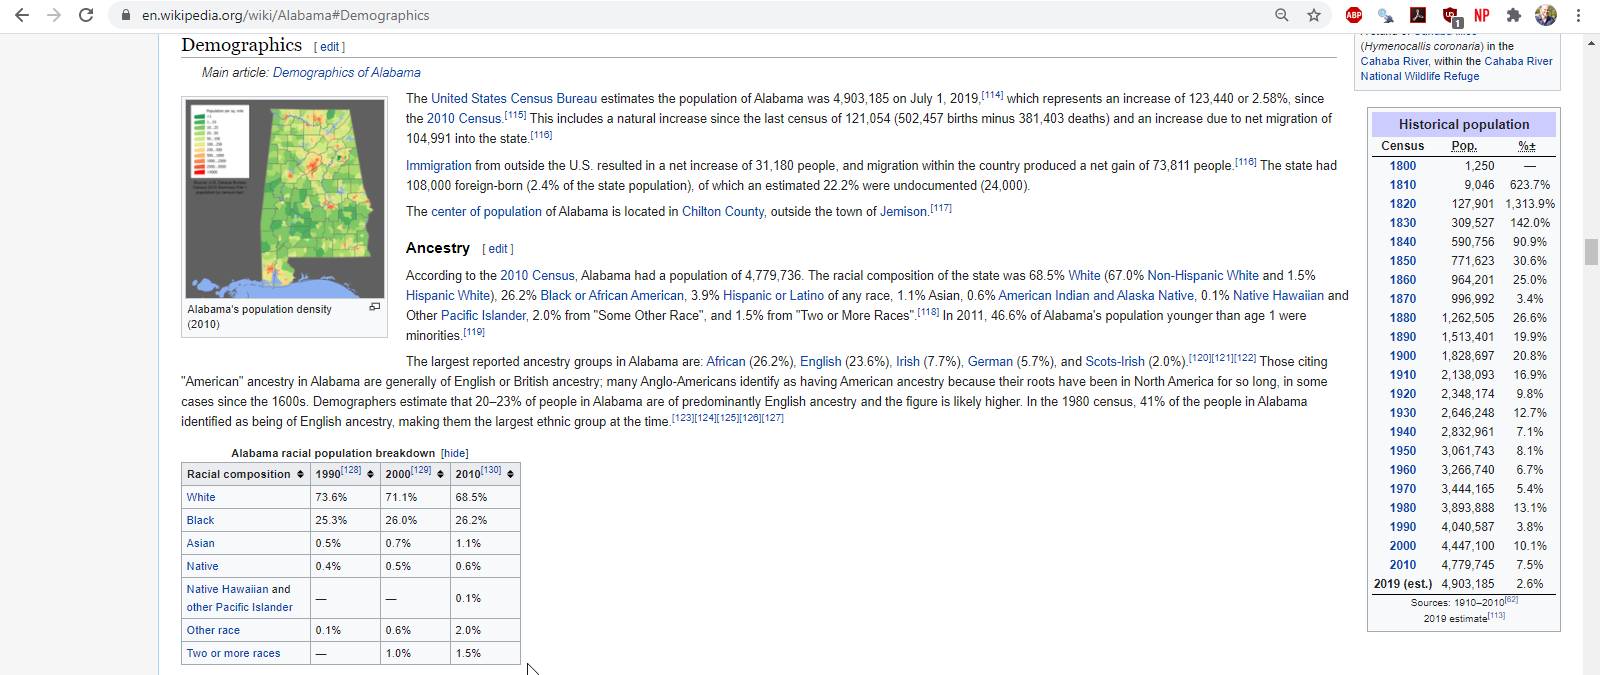
\includegraphics[width=22.22in]{src/images/alabama_demo_webpage} 

}

\caption{part of brainstorming is exploring different websites which may have the data you desire}\label{fig:unnamed-chunk-46}
\end{figure}

If we were to go to Georgia, we would notice that the web address is similar to Alabama, but since Georgia is also a country, the web address specifies that you are currently on the webpage for the state rather than the country. This effectively rules out editing the web address to iterate over each state.

If we broaden our search to `US States', we find a Wikipedia page with a list of each state. Each state has a hyperlink which takes us to the state's webpage with the demographic information we desire. Remember: hyperlinks are our friend! If they exist, we can scrape them, iterating over the web addresses to get data from each state. Let's use what we just learned to attain the web addresses for each state. We'll start with the web address containing a list of every state.

\begin{Shaded}
\begin{Highlighting}[]
\NormalTok{wiki_url <-}\StringTok{ "https://www.wikipedia.org"}
\NormalTok{states_url <-}\StringTok{ }\KeywordTok{str_c}\NormalTok{(wiki_url, }\StringTok{'/wiki/U.S._state#States_of_the_United_States'}\NormalTok{)}
\end{Highlighting}
\end{Shaded}

Let's use the page source to find where the hyperlinks exist in the HTML code. To do this, I am going to search for the phrase `The 50 U.S. states, in alphabetical order, along with each state's flag' in the page source since the list of states is just below this phrase.

\begin{figure}

{\centering 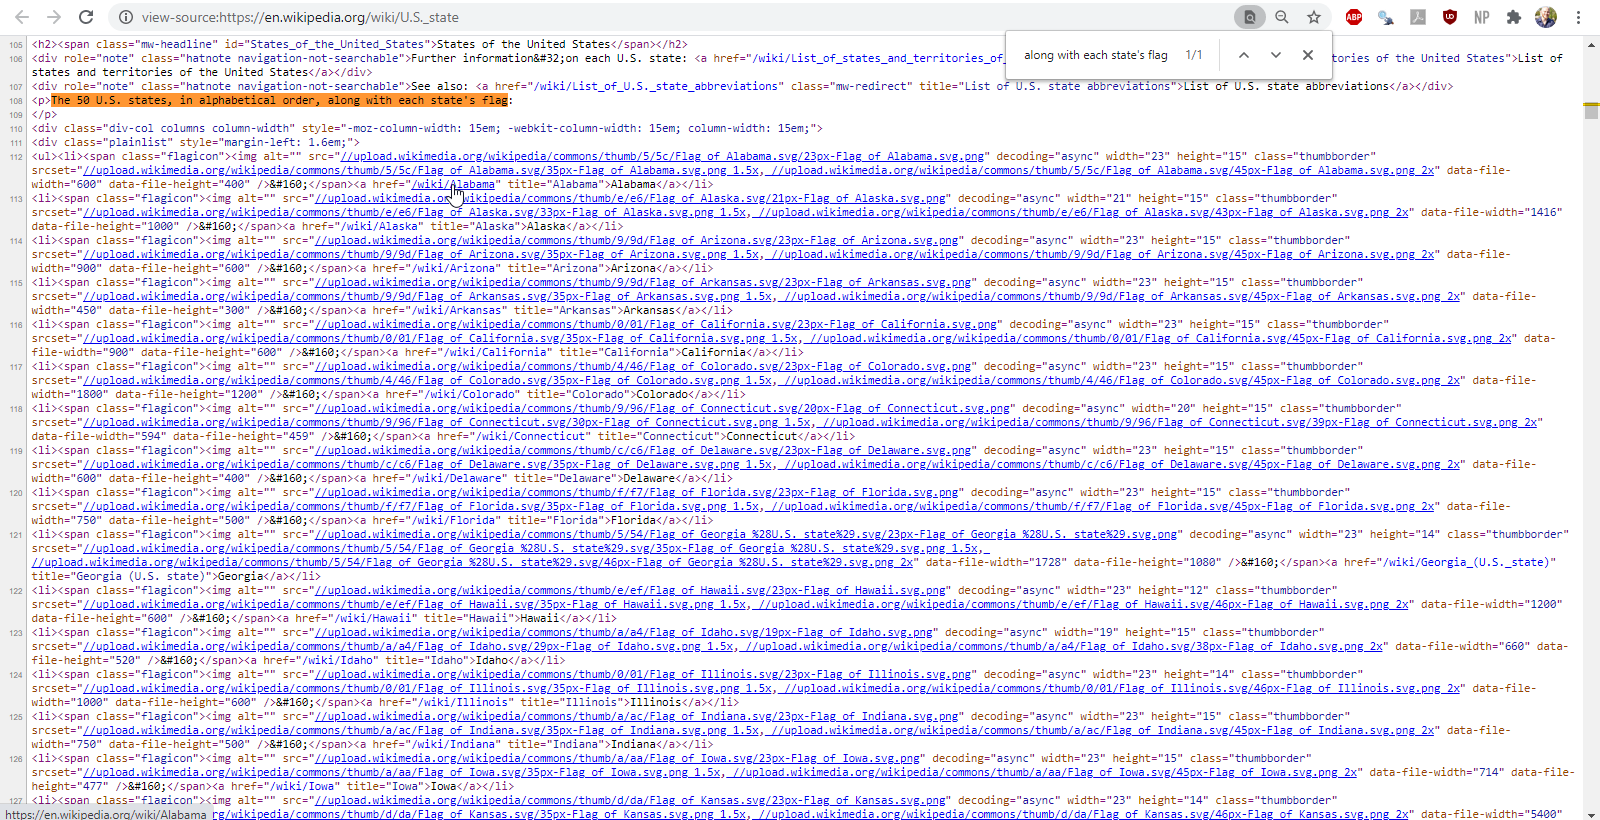
\includegraphics[width=22.22in]{src/images/usstates_page_source} 

}

\caption{finding the element containing the list of states with their cooresponding web addresses using the page source}\label{fig:unnamed-chunk-48}
\end{figure}

We find that the list of states, among other information, exists in an element tagged \texttt{div} with the attribute \texttt{class} set to an attribute value of \texttt{plainlist}. Within this node, the list of states exists in an element tagged \texttt{ul} and each state exists in an element tagged \texttt{li}. Within each state, the web address corresponding to that state's individual Wikipedia article is given in the \texttt{href} attribute to an element tagged \texttt{a}. Let's use this information to extract the web addresses corresponding to each state. We may also want to extract the state name which is the content of the element tagged \texttt{a}.

\begin{Shaded}
\begin{Highlighting}[]
\NormalTok{node_w_states <-}\StringTok{ }\NormalTok{states_url }\OperatorTok
\StringTok{  }\KeywordTok{read_html}\NormalTok{() }\OperatorTok
\StringTok{  }\KeywordTok{html_nodes}\NormalTok{(}\DataTypeTok{xpath =} \StringTok{"//div[@class='plainlist']"}\NormalTok{) }\OperatorTok
\StringTok{  }\KeywordTok{html_nodes}\NormalTok{(}\StringTok{'ul'}\NormalTok{) }\OperatorTok
\StringTok{  }\KeywordTok{html_nodes}\NormalTok{(}\StringTok{'li'}\NormalTok{) }\OperatorTok
\StringTok{  }\KeywordTok{html_nodes}\NormalTok{(}\StringTok{'a'}\NormalTok{)}

\NormalTok{ind_states <-}\StringTok{ }\KeywordTok{tibble}\NormalTok{(}\DataTypeTok{state =}\NormalTok{ node_w_states }\OperatorTok
\StringTok{                       }\KeywordTok{html_text}\NormalTok{(),}
                     \DataTypeTok{url =}\NormalTok{ node_w_states }\OperatorTok
\StringTok{                       }\KeywordTok{html_attr}\NormalTok{(., }\StringTok{'href'}\NormalTok{) }\OperatorTok
\StringTok{                       }\KeywordTok{str_c}\NormalTok{(wiki_url, .))}
\NormalTok{ind_states}
\end{Highlighting}
\end{Shaded}

\begin{verbatim}
# A tibble: 50 x 2
   state       url                                                
   <chr>       <chr>                                              
 1 Alabama     https://www.wikipedia.org/wiki/Alabama             
 2 Alaska      https://www.wikipedia.org/wiki/Alaska              
 3 Arizona     https://www.wikipedia.org/wiki/Arizona             
 4 Arkansas    https://www.wikipedia.org/wiki/Arkansas            
 5 California  https://www.wikipedia.org/wiki/California          
 6 Colorado    https://www.wikipedia.org/wiki/Colorado            
 7 Connecticut https://www.wikipedia.org/wiki/Connecticut         
 8 Delaware    https://www.wikipedia.org/wiki/Delaware            
 9 Florida     https://www.wikipedia.org/wiki/Florida             
10 Georgia     https://www.wikipedia.org/wiki/Georgia_(U.S._state)
# ... with 40 more rows
\end{verbatim}

Let's consider how we would scrape the racial demographics. Use either the selector gadget or the page source to identify where the desired table exists in the HTML code.

\begin{Shaded}
\begin{Highlighting}[]
\NormalTok{ind_states}\OperatorTok{$}\NormalTok{url[}\DecValTok{1}\NormalTok{] }\OperatorTok
\StringTok{  }\KeywordTok{read_html}\NormalTok{() }\OperatorTok
\StringTok{  }\KeywordTok{html_nodes}\NormalTok{(., }\DataTypeTok{xpath =} \StringTok{"//table[@class='wikitable sortable collapsible']"}\NormalTok{) }\OperatorTok
\StringTok{  }\KeywordTok{html_table}\NormalTok{() }\OperatorTok
\StringTok{  }\KeywordTok{as.data.frame}\NormalTok{()}
\end{Highlighting}
\end{Shaded}

\begin{verbatim}
                         Racial.composition X1990.128. X2000.129. X2010.130.
1                                     White      73.6%      71.1%      68.5%
2                                     Black      25.3%      26.0%      26.2%
3                                     Asian       0.5%       0.7%       1.1%
4                                    Native       0.4%       0.5%       0.6%
5 Native Hawaiian andother Pacific Islander          —          —       0.1%
6                                Other race       0.1%       0.6%       2.0%
7                         Two or more races          —       1.0%       1.5%
\end{verbatim}

In the next chapter, we will learn the tools to scrape the racial demographics for each state using the vector of web addresses we attained through this process as well as cleaning up these data according to tidy principles.

\begin{feedback}
Any feedback for this section? Click
\href{https://docs.google.com/forms/d/e/1FAIpQLSePQZ3lIaCIPo9J2owXImHZ_9wBEgTo21A0s-A1ty28u4yfvw/viewform?entry.1684471501=The\%20R\%20Community}{here}
\end{feedback}

  \bibliography{src/book.bib}

\end{document}
